\documentclass{report}
\usepackage{hyperref}
\usepackage[ngerman]{babel}
\usepackage{amsmath}
\usepackage{amsfonts}
\usepackage{amsthm}
\usepackage{tcolorbox}
\usepackage[a4paper, total={7in, 9in}]{geometry}
\usepackage[font={scriptsize,it}]{caption}
\usepackage{scrextend}
\usepackage{graphicx}
\usepackage{caption}
\usepackage{subcaption}
\usepackage[utf8]{inputenc}
\usepackage[T1]{fontenc}
\DeclareUnicodeCharacter{2212}{-}
\usepackage{verbatim}
\usepackage{tikz}

\tikzset{
  treenode/.style = {shape=rectangle, rounded corners,
                     draw, align=center,
                     top color=white, bottom color=blue!20},
  root/.style     = {treenode, font=\Large, bottom color=red!30},
  env/.style      = {treenode, font=\ttfamily\normalsize},
  dummy/.style    = {circle,draw}
}

\tikzstyle{level 1}=[level distance=3.5cm, sibling distance=3.5cm]
\tikzstyle{level 2}=[level distance=3.5cm, sibling distance=2cm]

% floating figure for column
\newenvironment{Figure}
	{\par\medskip\noindent\minipage{\linewidth}}
	{\endminipage\par\medskip}

\theoremstyle{definition}
\newtheorem{definition}{Definition}

\theoremstyle{example}
\newtheorem*{example}{Example}

\begin{document}

\begin{titlepage}
   \vspace*{\stretch{1.0}}
   \begin{center}
      \Large\textbf{eHealth - HS20}\\
      \large\textit{Pascal Brunner - brunnpa7}
   \end{center}
   \vspace*{\stretch{2.0}}
\end{titlepage}

% Beispiel Bild
%\begin{Figure}
%   \centering
%    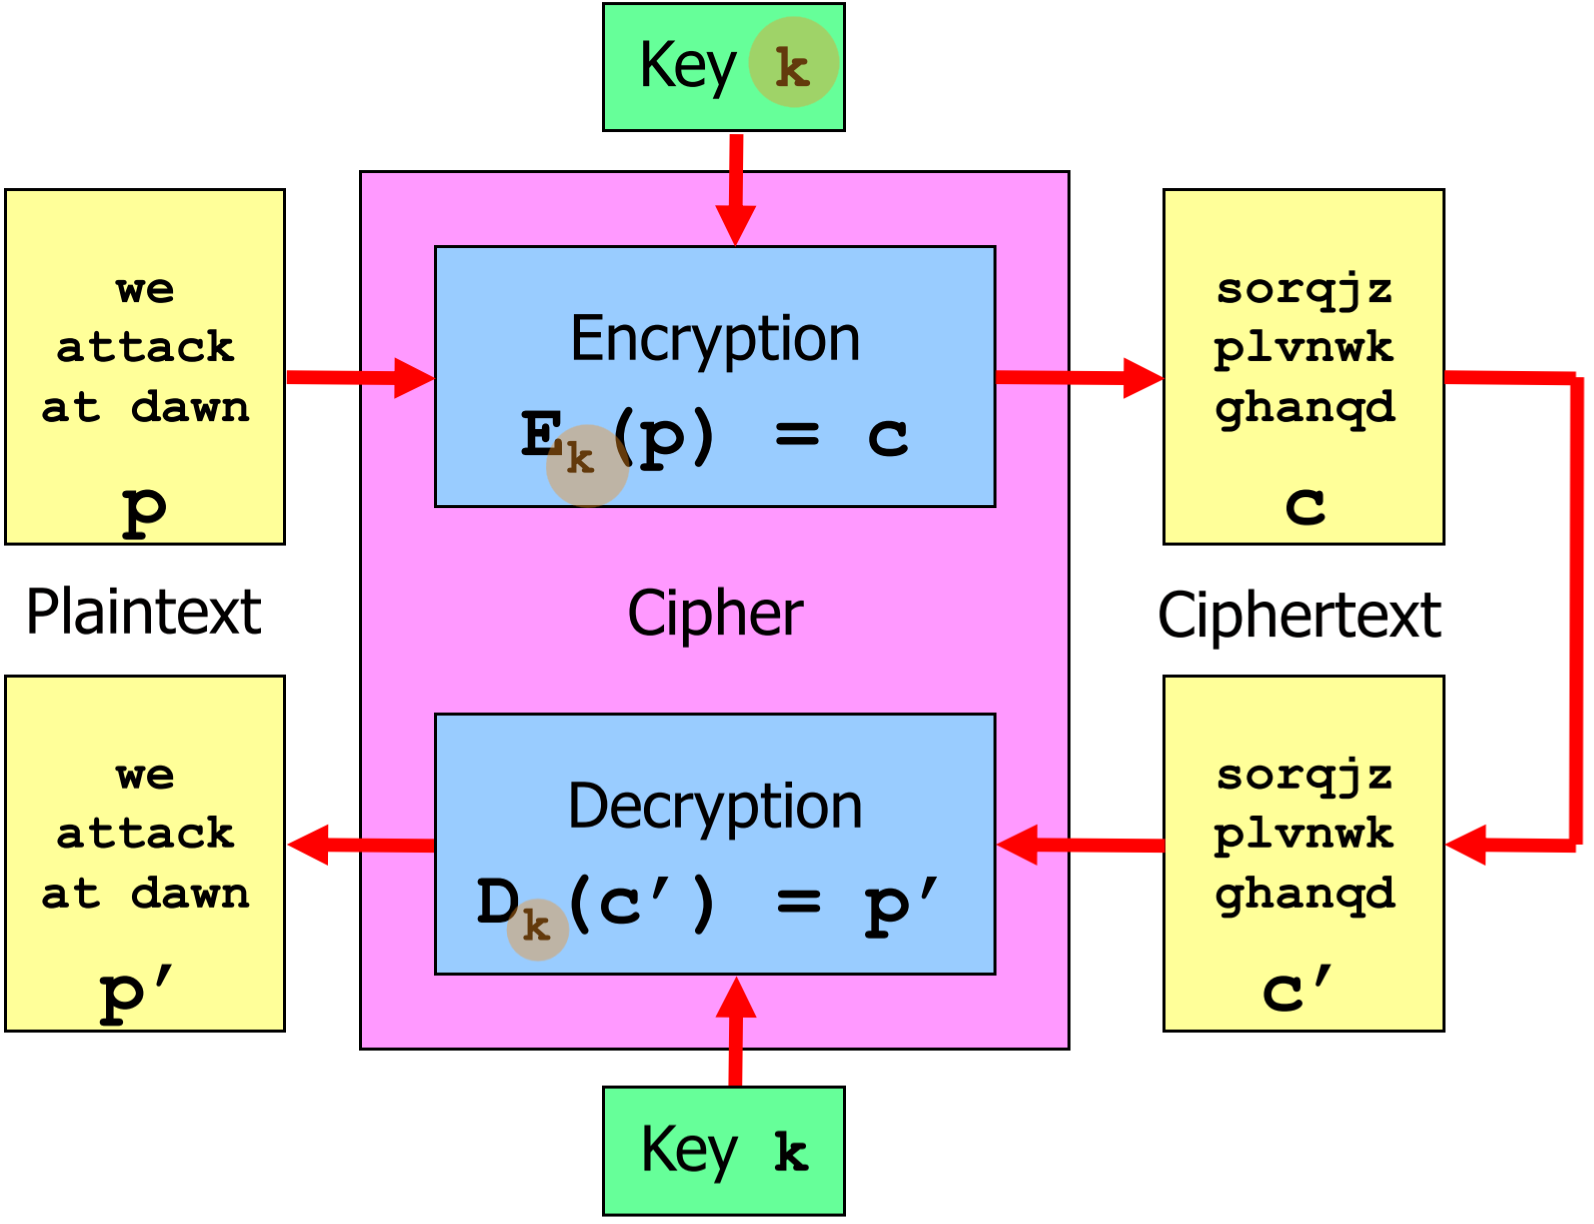
\includegraphics[width=150px]{img/BasicTerminologySecKeyCrypto.png}
%        \captionof{figure}{Basic Terminology basierend auf Secret Key Cryptography}
%        \label{fig:Basic Terminology}
%    \end{Figure}

\tableofcontents

\newpage

\chapter{Introduction}

\begin{Figure}
   \centering
    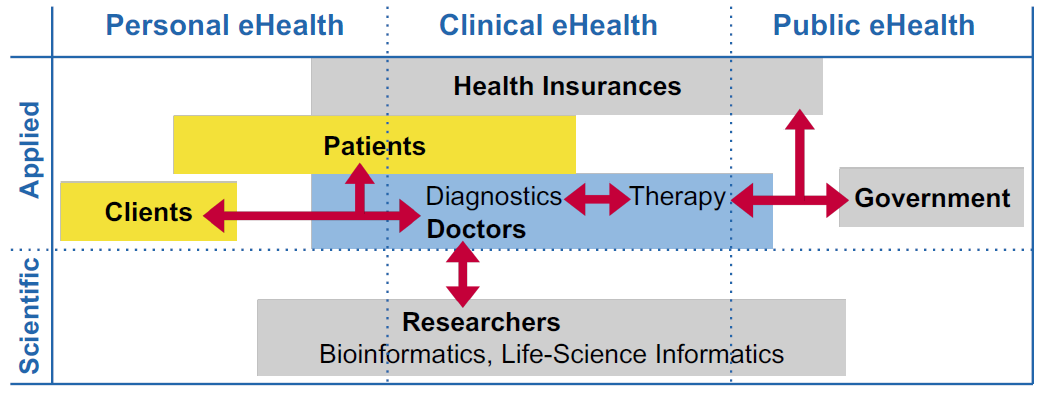
\includegraphics[width=150px]{img/domains.png}
        \captionof{figure}{Show the relationship between the different domains}
        \label{fig:eHealth domains}
    \end{Figure}

\section{What is eHealth?}
Supporting and improving the Health industry with ICT
\begin{itemize}
   \item ICT in healthcare
   \item Medical records and medical data standards
   \item Digital imaging
   \item Telemedicine / Telehealth
   \item more and more: Big Data is coming even in the healthcare
\end{itemize}

\textbf{Some numbers for Switzerland to start}
\begin{itemize}
   \item 80 billion CHF in 2016
   \item 30000 doctors
   \item 297 hospitals with 175000 employees, thereof 14000 hospital doctors
   \item 1700 pharamcies
   \item more than 2400 nursing homes and care organisation (e.g. Spitex) with 130000 employees
   \item more than 50 pharma companies with 40000 employees and with 6 mrd
   \item 61 insurance companies with 12000 employees
\end{itemize}

\textbf{What are the typical stakeholders?}
\begin{itemize}
   \item patients
   \item insurance companies
   \item pharma industry
   \item government
   \item care providers (hospitals, spitex, reha etc.)
   \item professional guilds (nurses, doctors etc.)
\end{itemize}

\textbf{public-private mix}
\begin{Figure}
   \centering
    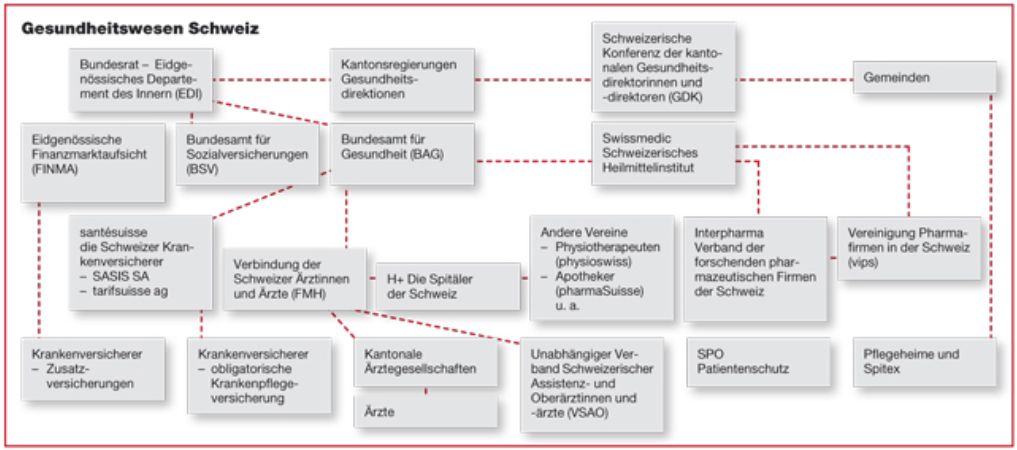
\includegraphics[width=150px]{img/publicprivatemix.png}
        \captionof{figure}{How does the public private mix look like in Switzerland}
        \label{fig:public private mix}
    \end{Figure}

\textbf{Vision of connected Healthcare}
\begin{Figure}
   \centering
    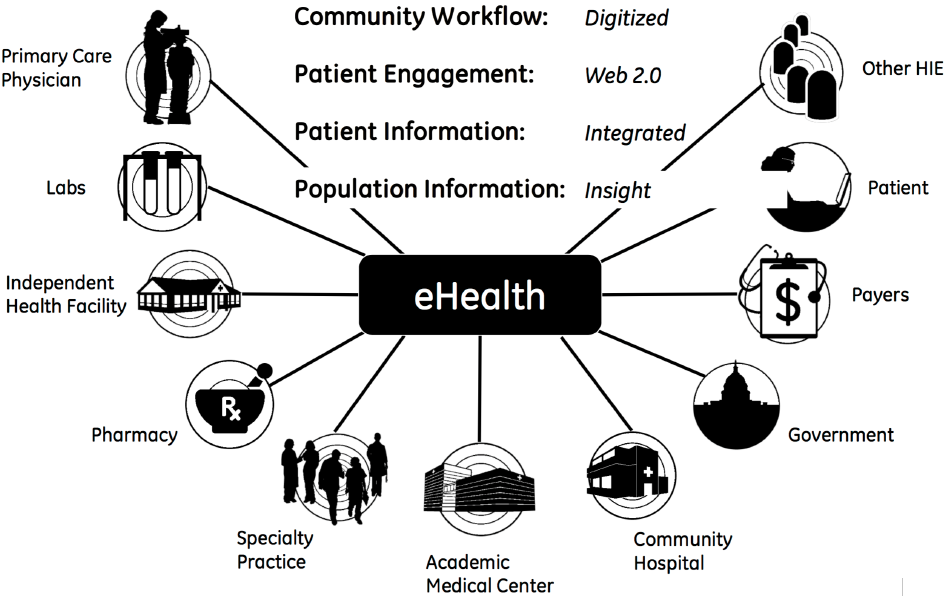
\includegraphics[width=150px]{img/vision.png}
        \captionof{figure}{how does the vision look like?}
        \label{fig:vision of healthcare in the future}
    \end{Figure}


    \subsection{Opportunities}
    It is definitely challenging, but the ultimate goal is to improve the quality of health care, researche and education in medicine and health\\
    \textbf{mid-term}
    \begin{itemize}
       \item Digital transformation: ICT tools AND processes
       \item Electronic Health records and data-driven services
       \item Digital integration, semantic interoperability, mHealth
    \end{itemize}

    \textbf{long-term}
    \begin{itemize}
       \item Individual, personalized medicine (genomics data)
       \item Longitudinal use of EHR data, data analytics, big data
       \item Knowledge management, medical DSS, deep learning
    \end{itemize}

\section{Personal Health}
\begin{itemize}
   \item Get greater quantities of health data to do predictive analytics
   \item Personal health record (Patientendossier)
   \item Quantify yourself $\rightarrow$ Fitness Apps
   \item Genomic medicine
   \item move towards personalized medicine
\end{itemize}

\section{Clincal Health}
\begin{itemize}
   \item Clinical information systems
   \item $\rightarrow$ Electronic medical records and medical vocabularies
   \item $\rightarrow$ Laboratory information systems
   \item Clinical decision-support systems
   \item Nursing informatics
\end{itemize}

\section{public Health}
\begin{itemize}
   \item Regulations, laws and standards $\rightarrow$ Legal, Quality, Social, Health insurances
   \item Epidemics, travel medicin $\rightarrow$ Ebola, Zika, covid $\Rightarrow$ Analysis the data to identify diseases within a region and with that to get a public health alert
   \item 
\end{itemize}

\section*{Why is it important?}
\begin{itemize}
   \item Healthcare in developed countries is under the biggest 5 industry sectors
   \item Helathcare in developed countries counts for about 10 \% of Gross Domestic Product (BIP)
   \item costs are growing $\rightarrow$ grow rate is higher than GDP growth
   \item In Switzerland we pay 12.2 \% of all the money (GDP) for healthcare
   \item The Age structure is changing $\rightarrow$ Higher life expectancy (we get older than 80)
   \item We die after long period with chronic diseaes and this has changed compared to years ago - this is the bad news about living longer
   \item The costs of healthcare has increased dramatically $\rightarrow$ Ausgaben wurden seit 1969 verdopplet von 6 auf 12 Prozent
   \item 
\end{itemize}

\section{General Practitioner (Hausarzt)}
   \subsection{a day in a life}
   \begin{itemize}
      \item Family doctor or physician
      \item typically works in private or group practice
      \item provides diagnosis and care for patients in routine cases $\rightarrow$ ambulant care
      \item usually refers people to specialists when they need specific types of treatment
      \item has receptionsst and physician assistant
   \end{itemize}

   \subsection{typical workflow}
   \begin{enumerate}
      \item Pre-visit: Appointment scheduling and information collection
      \item Check-in: patient check-in and payment collection/Health insurance registration
      \item Control: rooming, measuring vital signs, patient examination, prescription and result documentation $\rightarrow$ optional there are some extra lab-tasks e.g. blood test 
      \item Check-out: patient checkout
      \item Post-visit: coding and billing / Reviewing Test results
   \end{enumerate}

   \subsection{Clincal Tools}
   Paper- or IT-based, whether what is used, there are medical records used
   \begin{itemize}
      \item Screening for illness and disease $\rightarrow$ identify at-risk patents
   \end{itemize} 

   \subsection{Medication Management}
   \begin{itemize}
      \item Medication errors are the most frequent source of preventable medical errors
      \item Medication Administration Record 
      \item Electronic Medication Administration records
      \item Adverse Drug Event $\rightarrow$ side effect or complication
      \item Transition points $\rightarrow$ times when patients move from one location to another
      \item Medication reconcilation $\rightarrow$ comparing patients list of medications at admission with medications ordered during hospital stay
      \item order sets $\rightarrow$ standardized list of orders for a specific diagnosis e.g. heart disease
   \end{itemize}

      \subsubsection{What could go wrong?}
   \begin{itemize}
      \item Drug-Allergy Conflic
      \item Drug-Disaese Conflict
      \item Incorrect Dosage
      \item Incorrect Duration
      \item Drug-Pregnancy Conflict
      \item Drug-Age Conflict
      \item Drug-Gender Conflict
      \item Drug-Drug Conflict
   \end{itemize}
   $\rightarrow$ This could be checked by a electronic drug databases to reduce the errors

   \subsection{Coding and reimbursement}
   \begin{itemize}
      \item Documentation and coding plays a major role in whether a payer (health insurance) approves claims and reimburse the physician
      \item Computer-assisted coding uses software to faciliate claim processiong
      \item typically country-specific $\rightarrow$ in Switzerland TARMED (Tarif Médicaux)
   \end{itemize}
   
      \subsubsection{TARMED}
      \textbf{Overview:}
      \begin{itemize}
         \item TARMES is the swiss standard tarif for medical and paramedical services provided in medical practices and hospitals
         \item since 2004 in every canton
         \item TARMED tariff comprises about 4600 positions
         \item Pricing of medical services is calculated consistently throughout Switzerland with so-called tax positions
         \item However, the amount of remunerations per tax point varies from canton to canton
         \item These codes from TARMED we will find on our bills from the doctor, 
      \end{itemize}

\section{Current situation / status of healthcare industry}
\begin{itemize}
   \item Physician: still heavily paper-based $\rightarrow$ to record, store and communicate in hand-written as well as with fax
   \item Hospitals: core ICT in use $\rightarrow$ nevertheless there is space for improvement
\end{itemize}

   \subsection{Why does healthcare lack in ICT}
\begin{itemize}
   \item complexity of care / of healthcare ecosystem $\rightarrow$ many stakeholders, large number of small org
   \item Incentives are misaligned $\rightarrow$ Goals are different; higher quality may not result in more customers
   \item Data entry effort vs. personal benefit
   \item Network externality / missing network effects
\end{itemize}

\section{Telehealth}
Telehealth includes the use of technology to access remote health information, diagnostic imgaes and education
\begin{itemize}
   \item Email communication
   \item Refilling prescriptions
   \item Registering patient
   \item Scheduling appointments
\end{itemize}

\section{Telemedicine}
The use of medical information exchanged from one site to another via electronic communications
\begin{itemize}
   \item Provision of healthcare services through the use of ICT, in situation where patient and health professional are \textbf{not} in the same location
   \item Specialist referral
   \item Remote patient monitoring
   \item Store and forward digital images
   \item Interactive videoconferencing
   \item Telesurgery
\end{itemize}

\chapter{Healthcare Information Systems (HIS)}

\textbf{Definition Hospital}:\\
\textit{A hospital is ahealth care instituation with an organized medical and professional staff, and with permanent facilities
that include in-patient beds. provides medical, nursing and other health-related services to patients}\\
\textbf{functions}
\begin{itemize}
   \item preventive functions
   \item curative functions
   \item trainings functions
   \item reasearch functions
\end{itemize}

\section{Categories of healthcare organizations}

   \subsection{Classifcation of health care organizations}
   \begin{itemize}
      \item By length of stay
      \subitem Short stay (less 24hrs), traditional acute care (1-30d), long-term care 
      \item By type of ownership
      \subitem government vs. non-government 
      \item By type of services
      \subitem general vs. specialty, community vs. teritary, in-home vs. ambulant 
   \end{itemize}

   \subsection{Types of Healthcare organizations}
   \begin{itemize}
      \item General hospital
      \subitem medical, surgical, emergency 
      \item Specialty hospital
      \subitem Psychiatric, women's, children's hospital 
      \item teritary hospital
      \subitem complex and unsual problems 
      \item sub-acute care
      \item in-home health services
   \end{itemize}

   \subsection{Grouping of hospital services}
   \begin{itemize}
      \item Administrative services $\rightarrow$ Management, HR
      \item Informational services $\rightarrow$ billing, education, IT
      \item therapeutic services
      \item diagnostic services
      \item support services
   \end{itemize}

   \subsection{Patient Flow in a hospital}
   \begin{enumerate}
      \item Registration and scheduling
      \item nursing situation
      \item ancillary services
      \item surgey
      \item ... until patient is ready to be discharged
   \end{enumerate}
   \begin{Figure}
      \centering
       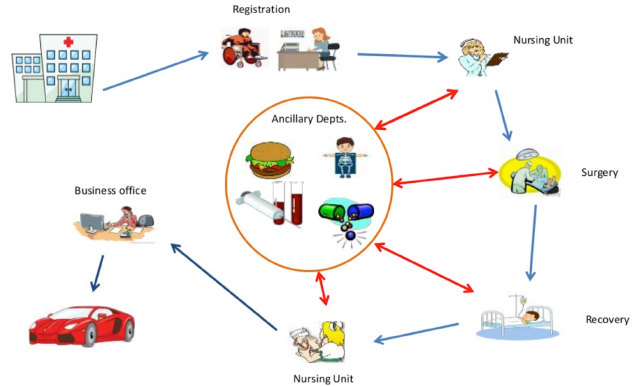
\includegraphics[width=150px]{img/inpatienFlow.png}
           \captionof{figure}{how does the inpatient flow look like}
           \label{fig:inpatient Flow}
       \end{Figure}

\section{Information systems in healthcare organizations}

\subsection{Complexity of ICT at hospital}
\begin{itemize}
   \item Practitioners' offices typically maintain one Clinical information system
   \item have numerous clinical information systems (Laboratory, pharmacy, radiology systems etc.)
   \item Need for interoperability and integration
\end{itemize}
$\Rightarrow$ A HIS is really complex not only in the functions but also in the GUI
\begin{Figure}
   \centering
    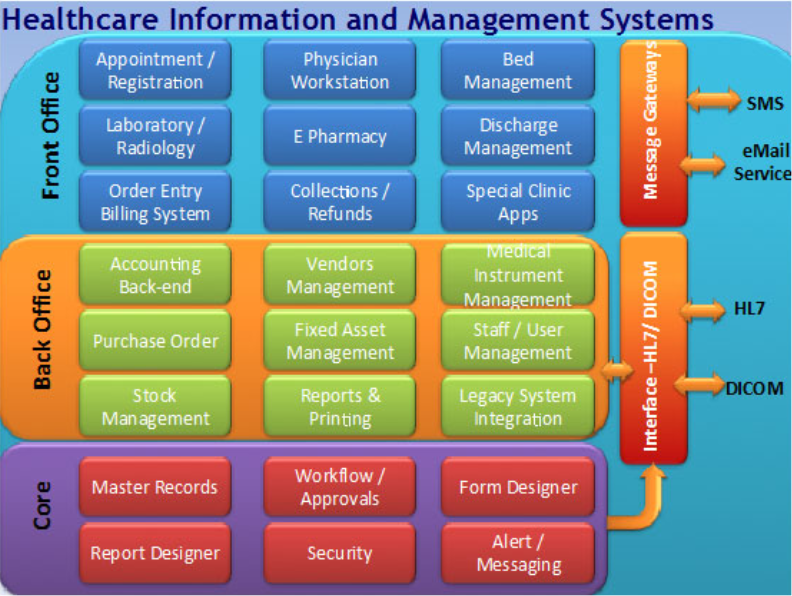
\includegraphics[width=150px]{img/HIS.png}
        \captionof{figure}{Healthcare information and management systems}
        \label{fig:HIS}
\end{Figure}

\subsection{Main Functions from a HIS}
There are two types
\begin{itemize}
   \item clincal support
   \item Administrative support
\end{itemize}

We need all information and have directly access to the information, to get a better documentation and improve the quality of care.\\ 
Especially to reduce to errors in daily business and improve the productivity and efficiency.


\subsubsection{Clincal Support}
\textbf{Nursing}\\
Support the daily business of a nurse e.g. view and update vital data, access to drug info\\
\textit{Goal:} Documentation access to info, productivity and communications, regulatory compliance\\

\textbf{Monitoring}\\
monitor the patients and alert immediately if there is an abnormal finding e.g. real-time monitoring, automatically feeding into the CIS\\

\textbf{Order Entry}\\
Direct entry of orders for medication and transmit orders online (e.g. pharmacy, Laboratory, radiology, social services, ...)\\

\textbf{Laboratory}\\
so-called \textit{Laboratory Mangement System} to provide
\begin{itemize}
   \item Manage lab test
   \item alert if a test results is critical
   \item Send results to CIS
   \item Accept inputs from bedside devices
   \item Use rules to order additional tests
   \item Address issues such as turn-around time, duplicates, errors
\end{itemize}
\textit{LOINC Standard} Logical Observation Identifiers Namens and codes\\

\textbf{Radiology}\\
Should provide the functions to support the daily business such as
\begin{itemize}
   \item allow direct order
   \item Scheduling diagonstic test
   \item generate client instructions
   \item permit transcription of results
   \item provide picture archiving
   \item generate charges once procedures are done
\end{itemize}
\textit{Picture Archiving and Communication Systems (PACS)}: Images from X-Ray/CT/MRI devices transferred PACS which is linked directly to the CIS. And provide directly access to results and searching\\

\textbf{Pharmacy} (eMedication / ePrescription)\\
\begin{itemize}
   \item provide checks in order
   \item administration process using evidence-based guidelines
   \item Barcode and RFID Medication administration
   \item Dispensing systems
   \item Use lab results, allergy and interaction information from CIS
   \item track medication use, costs and billing information
\end{itemize}
\textit{Electronic Medication Administration Records (eMAR)} the main goal is to eliminate errors.

\subsubsection{Administrative Information Systems}
It is a very often scenario that a hospital runs two different system, one for the CIS and one for the Admin-part
\textbf{Patient and Client Registration}\\
\begin{itemize}
   \item admission, discharged and Transfer (ADT) systems
   \item Collect and sotre demographic and insurance data
   \item critical to opersionts to ensure correct patient identification
   \item One of the most important part is how to identify the patient (Barcode etc.)
\end{itemize}

\textbf{Financial Systems}\\
\begin{itemize}
   \item Charge all services
   \item provide data for insurance
   \item financial controlling
   \item generate reports
\end{itemize}

\textbf{Payroll and Human Resources}\\
\begin{itemize}
   \item Payroll
   \item Contracting
   \item Career planing
   \item Physical access control (key, badge etc)
\end{itemize}

\textbf{Risk Management}\\
\begin{itemize}
   \item risk monitoring
   \item reduce risk
\end{itemize}

\textbf{Quality Assurance}\\
\begin{itemize}
   \item Management Cockpit
   \item Decision Support Systems
\end{itemize}

\textbf{Contract Management}\\
\begin{itemize}
   \item provide visibility and control to negotiate better contract with vendors etc.
\end{itemize}

\textbf{Scheduling Systems}\\
\begin{itemize}
   \item Planning appointments
   \item Staff Planning
   \item insurance approval
   \item charging information
\end{itemize}

\textbf{Other Admin Systems}\\
\begin{itemize}
   \item IT Security Management
   \item Facility Management
   \item Roles and Access Rights Mgmt
\end{itemize}

$\Rightarrow$ The IT-Security Part is one of the most important and fragile parts in a hospital. If a hospital gets hacked, there are a lot of consequences and it can decide between life and death.

\chapter{EHR}
Electronic Health Record conforms to nationally recognized interoperatibility standards, \textbf{across more} than one organization

\section{Electronic Medical Record}
\begin{itemize}
   \item typically created in hospitlas and ambulatory environment using HIS
   \item Case-based: single encounter of treatment
   \item structured data (predefined format with discrete data encoding)
   \item to provide patient care, communication, legal documentation, billing etc.
   \item Content examples: identification, problem-list, progress notes, lab reports, discharge summary
\end{itemize}

\section{Adaoption Model}
\begin{enumerate}
   \item Stage 0
   \subitem all paper based 
   \item Stage 1
   \subitem all three major ancillaries installed - laboratory, pharmacy and radiology 
   \item Stage 2
   \subitem 
   \item Stage 3
   \subitem Clinical documentation installed
   \subitem First Level of clinican decision support is implemented to conduct error
   \subitem Image access from picture archive and communication system (PACS)
   \item Stage 4
   \item Stage 5
   \subitem closed loop mediciation administration environment is fully implemented
   \subitem Using eMAR (barcode) 
   \item Stage 6  
   \item Stage 7
   \subitem fully paperbased   
\end{enumerate}

\section{EHR}
\begin{itemize}
   \item Comprehensive lifetime health record
   \item manages episodic and longitudinal information
   \item patient-oriented health data
\end{itemize}
\subsection{purpose}
\begin{itemize}
   \item Continuity of care documentation (CCD)
   \item engage patients and Family
   \item maintain privacy and security of patient health information
   \item improve care coordination and population and public care
\end{itemize}
\subsection{Content of EHR}
\begin{itemize}
   \item personal and family health data
   \item vaccinations (Impfbuch)
   \item Allergies
   \item medication record
   \item health data
   \item fitness and mental data (sensors, self-recorded)
   \item physician's order, treatment plans, diet plans
   \item medical images and reports
   \item laboratory reports
   \item consents and authorization forms (Stoffwechsel)
   \item Pathology and operative reports
   \item Health history summary, dashboard, analytics, visualisation
\end{itemize}
\subsection{Issues in EHR Implemntation}
\begin{itemize}
   \item EHR Infrastructure
   \item Common Vocabulary
   \item Data Integrity
   \item Data ownership
   \subitem Who is the owner of the data
   \subitem Patients own their data and should have full access 
   \item Privacy and Confidentiality
   \item Development and Maintance costs
   \subitem Who will pay? government, insurances, patients?
   \item caregiver resistance
   \item political System
\end{itemize}

\chapter{Health Data - Standards and Ontologies}

\section{HIS related}

\subsection{Challenges}
\begin{itemize}
   \item Hospital is a huge organisation $\rightarrow$ many departments, people, stakleholders and activities
   \item demand for good information $\rightarrow$ the right content in the right time at the right time to a specific user
   \item distribution of data and knowlege $\rightarrow$ many different sources, location and systems create a lot of data (structured and unstructured)
\end{itemize}

\subsection{Usability Issues}
\begin{itemize}
   \item Interference with patient visit
   \item Lack of system-design support for team-based care
   \item care coordination due to lack of data interoperability
   \item increased cognitive workload for physicians
   \item lack of product modularity to support unique needs
   \item lock-in to systems
   \item communicating with patients in a changing digital landscape
   \item insufficient support for enduser
\end{itemize}


\section{Types of data}
\textbf{Clinical Data}
\begin{itemize}
   \item clinical or health-related information used by providers in diagnosing, treating and monitoring
   \item case-based: illness, accident
   \item life-cycle-oriented: medical health record
\end{itemize}

\textbf{administrative Data}
\begin{itemize}
   \item primary purposes on the administrative data side is billing
   \item dealing with diagnosis codes and procedure codes $\rightarrow$ TARMED or SwissDRG
\end{itemize}

\section{Entering Data into a HIS}
There a various ways to enter the data into a HIS. The data will be enter by a desktop computer (after consultation or discharge) or mobile device (bed-side)
\begin{itemize}
   \item manual typing
   \item clinical templates
   \item dictation and transcription
   \item voice recognition
   \item scanning and OCR
   \item touchscreen
\end{itemize}

\section{Metadata}
data about data - there are different levels of metadata and therefore different Complexity
\begin{itemize}
   \item Schema $\rightarrow$ Definition of data format (e.g. XML Schema)
   \item Vocabulary $\rightarrow$ allowed values, code translation
   \item Classifcation $\rightarrow$ topic-oriented type hierachy
   \item Taxonomy $\rightarrow$ controlled vocabulary with structured directory of terms
   \item Thesaurus $\rightarrow$  map words to concept
   \item Ontology $\rightarrow$ Model of a domain with rules and it is a knowledge representation which is machine-readable 
\end{itemize}

\subsection{Semantic gap}
Since words has different meaning in a specific context sometimes it is not clear what is meant. Therefore it's a \textbf{semantic gap} between words and concept\\
e.g.: Double Bass = Upright Bass = Contrabass (synonym) or  fruit $\leftarrow$ Apple $\rightarrow$ Company\\
$\Rightarrow$ Thesauri and onotlogies manage semantic

\subsection{Categorization}
Generalization vs. Specialization $\rightarrow$ we typically learn basic level (e.g. Chair, Table) categories first\\
\begin{itemize}
   \item we get more precise with subcategories $\rightarrow$ Hyponym (Unterbegriffe) and subordinate (untergeordnet) e.g. dining chair, kitchen table
   \item we get more abstract with supercategories $\rightarrow$ hypernyms (Oberbegriff) and superordinate (übergeordnet) e.g. furniture
\end{itemize}

\section{Clinical Information Standards}

\subsection{Classication Systems}
\begin{itemize}
   \item International Classifcation of Diseases, Ninth Revision (ICD-9)
   \item International Classifcation of Diseases, Tenth Revision (ICD-10)
   \subitem Current Procedural Terminology (CPT)
   \subitem Healthcare Common Procedures Coding System (HCPCS), Level II
   \item Anatonmical Therapeutic Chemical (ATC) Classifcation
   \subitem Classifies therapeutic drugs 
\end{itemize}

\subsection{Clincal Vocabularies and Ontologies}
\begin{itemize}
   \item SNOMED-CT - \textit{Systematzied Nomenclature of Medicine Clinical Terms}
   \subitem Identifies atomic entities such as chemicals, diagnoses, findings, anatomic sites and organisms
   \item LOINC - \textit{Logical Observation Identifiers Namens and Codes}
   \subitem Identifies laboratory tests, clinical variables and survey instruments
   \subitem for recording single observation, measurement, test result 
   \item UMLS - \textit{Unified Medical Language System}
   \subitem By the US National Library of Medicine (NLM) 
   \item RxNorm - \textit{US specific terminology, part of UMLS}
   \subitem Identifies the clinical drug and its component, ingredients, dose form etc. 
\end{itemize}

\subsubsection{SNOMED-CT}
\begin{itemize}
   \item Systematzied Nomenclature of Medicine Clinical Terms
   \item Codes, terms, synonyms and definitions covering anatomy, diseases, findings, procedures etc
   \item globally recognized ontology
   \item needs license $\rightarrow$ Siwtzerland applied to become offical member (started first a test phase)
\end{itemize}
\textbf{SNOMED-CT Coding Clinical Terms Identifer (SCTID)}\\
\begin{itemize}
   \item SNOMED-CT Clinical Terms Identifer (SCTID)
   \item Sequence of 6 to 18 digits that identifies a component
   \item directed acyclic graph
\end{itemize}
\begin{Figure}
   \centering
    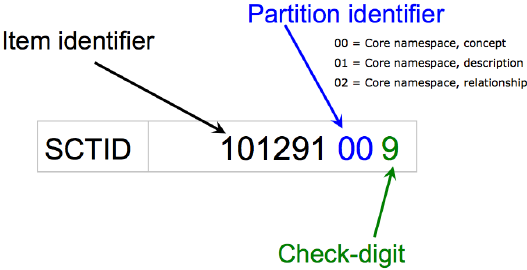
\includegraphics[width=150px]{img/SCTID.png}
        \captionof{figure}{example for SCTID}
        \label{fig:example for SCTID}
\end{Figure}

\textbf{SNOMED-CT Ontology Structure}
\begin{itemize}
   \item Combing isa-hierarchy and attribute relations
   \subitem ISA classification hierarchy
   \subitem Attribute relations $\rightarrow$ cause, finding, site(anatomy), severity 
   \item Reference Sets (RefSets)
   \subitem Groups of SNOMED components to be used for a patricular purpose 
\end{itemize}

\begin{Figure}
   \centering
    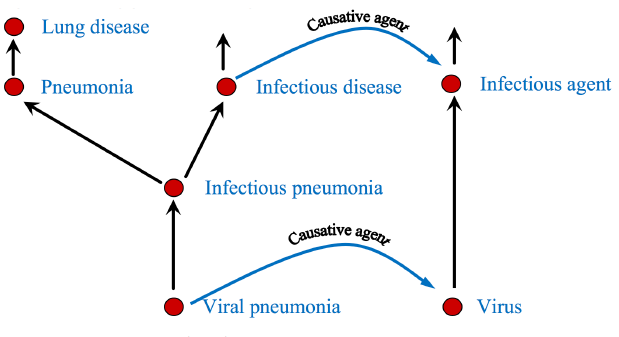
\includegraphics[width=150px]{img/SNOMED Ontology.png}
        \captionof{figure}{SNOMED-CT Ontology Structure}
        \label{fig:SNOMED-CT Ontology Structure}
\end{Figure}

\subsubsection{LOINC}
\begin{itemize}
   \item Logical Observation Identifiers Namens and Codes
   \item A universal code system for tests, measurements and obervations
   \item LOINC is a database with universal codes and names for 71'000 observations identifying laboratory test, clinical measures and survey instruments
   \item Carries information about each test and measurement
   \item Represents a measurement, question or observable and consists of
   \subitem LOINC Code (Numeric with dash and check-digit)
   \subitem LOINC Name (what SNOMED CT would call a term) 
   \item is an international standard $\rightarrow$ translated into 14 languages
   \item license for free use
\end{itemize}

\textbf{The six Part Types:}
\begin{itemize}
   \item Component or Analyte $\rightarrow$ What is being measured
   \item Property $\rightarrow$ the characteristic of how it is being measured
   \item time $\rightarrow$ when the measurement is being completed
   \item System $\rightarrow$ Where the analyte originates
   \item Scale $\rightarrow$ which way will the test result be expressed
   \item method $\rightarrow$ what method was used to make the measurement
\end{itemize}
\textit{example:} Sodium:SCnc:Pt:Ser/Plas:Qn \\
\begin{itemize}
   \item analyte is Sodium
   \item measured by substance concetration
   \item measured at onepoint in time
   \item measured on either serum or plasma
   \item result is quantitative
   \item in this example, method used is not included
\end{itemize}

\subsubsection{ATC Classification System}
\begin{itemize}
   \item Anatomical Therapeutic Chemical (ATC)
   \item Classification of active ingredients of drugs $\rightarrow$ according to the organ or system on which they act
   \item 14 top classes
   \item controlled by the WHO
\end{itemize}

\subsubsection{Swiss Standards}
\begin{itemize}
   \item AIPS (Arzneimittel-Informations-Publikations-System)
   \subitem By Swissmedic
   \subitem electronic drug index
   \item hospINDEX database
   \subitem catalog of pharmaceutical products registered in Switzerland
   \subitem used by HIS for computerized physician order entry (CPOE)
   \item DRGs: Diagnosis-Related Groups (Fallgruppen)
   \subitem Classication system used for the financing of hospital stays (Fallpauschalenkatalog)
   \subitem Basis for reimbursement
   \subitem used in hospital for budget planning
   \subitem developed in USA (70s) 
   \item SwissDRG is part of the health insurance law reform
   \subitem Based on the German G-DRG
   \subitem since 2012 with fix rates
   \subsubitem before: financing of daily costs
   \subsubitem after: financing per case by fixed rates
   \subitem reduce costs by encouraging hospitals to adopt best practices  
\end{itemize}

\subsection{Messaging Standards}
\begin{itemize}
   \item Health Level Seven (HL7)
   \subitem Interoperability specification for health and medical transaction (HL7 v2, HL7 v3)
   \subitem Clinical Document Architecture (CDA), part of HL7 v3
   \subitem Continuity of Care Document (CCD): medical summaries as CDA 
   \item Digital Imaging and Communications in Medicine (DICOM)
   \item Picture Archiving and Communication System (PACS)
   \item National Council for Prescription Drug Program (NCPDP)
   \item The INstitute of Electrical and Electronics Engineers 1073 (IEEE1073)
   \subitem Medical device communication standard 
\end{itemize}

\subsection{ICD-10}
\begin{itemize}
   \item \textbf{I}nternational \textbf{C}lassification of \textbf{D}iseases
   \item Maintened by the World Health organization (WHO)
   \item ICD-10-CM codes used in documenting diagnoses (cm = clinical modification) published in 1994 $\rightarrow$ 3-7 characters in length and total about 68'000 diagnoses
   \item ICD-10-PCS are the procedure codes $\rightarrow$ 7 characters in length (alphaNum) and total about 87'000 procedures
   \item Final version of ICD-11 endorsed in 2019 by WHO
\end{itemize}

\subsubsection{Codes in ICD-10}
These codes are very specific, which means
\begin{itemize}
   \item Clinical data with high specificty 
   \item improved care management of beneficariaries
   \item reliable and robust clinical data that can be used to make intelligent, data driven decision
   \item more accurate payments
   \item reduced number of miscoded, rejected and improper reimbursement claims
   \item better data for fraud and abuse monitoring
   \item better understanding of healthcare outcomes
   \item codes to address global dieases emergencies
\end{itemize}

\chapter{HL7 und HL7 FHIR}

\section{Interoperability}
inter: zwischen, opera: arbeit $\rightarrow$ this happens in different levels
\begin{itemize}
   \item technical
   \item syntactically
   \item semantically
   \item crossdomain
\end{itemize}

\section{The HL7 v2.n Messaging Standard}
\begin{itemize}
   \item Easy to use and understand
   \item Based on an implicit information model
   \item also an international use
   \item Works well withing a single enterprise
   \item does not work well when sender and receiver are not connected
   \item available with delimiter or with XML syntax
   \item Messages initiated by trigger events
\end{itemize}

\section{HL7 FHIR STU}
\begin{itemize}
   \item \textbf{F}ast $\rightarrow$ faster to develop, learn, implement
   \item \textbf{H}ealthcare
   \item \textbf{I}nteroperabiliity
   \item \textbf{R}esources $\rightarrow$ Resources as bricks, web technology (RESTful API)
\end{itemize}

\chapter{IHE}
\begin{itemize}
   \item IHE is an iniative by healthcare professionals and industry to improve the way computer systems in healthcare share information
   \item Promotes the cooridnated use of established standards such as DICOM and HL7 to address specific clincal needs in support of optimal patient care
   \item IHE for
   \subitem Clinicans
   \subitem IT professionals
   \subitem Healthcare Administrators
   \item IHE is
   \subitem NOT a standardization body
   \subitem NOT a certification body 
\end{itemize}

\begin{Figure}
   \centering
    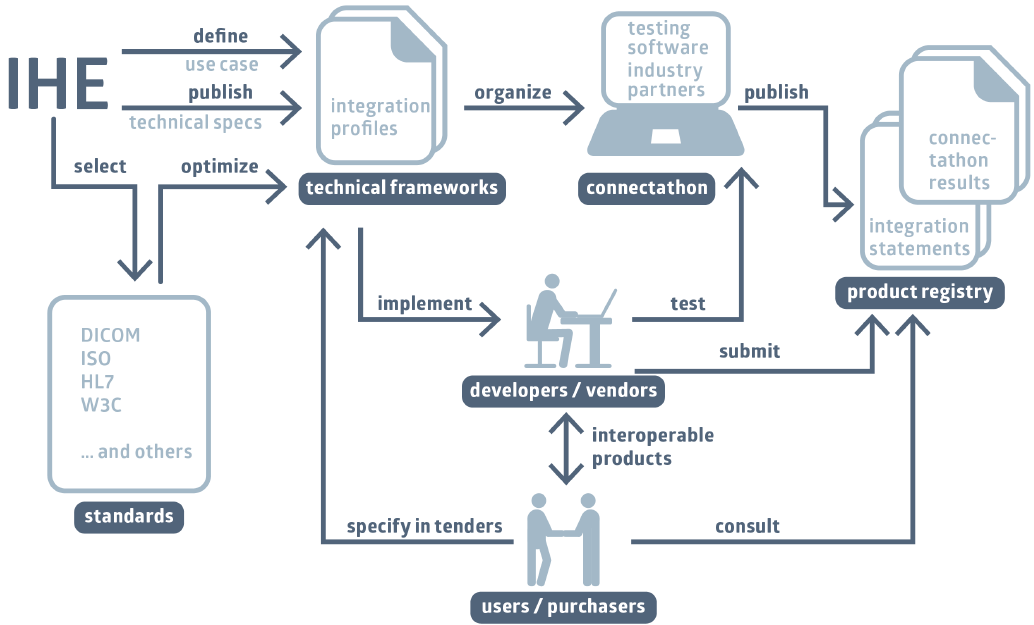
\includegraphics[width=150px]{img/IHE.png}
        \captionof{figure}{Descirption IHE}
        \label{fig:Descirption IHE}
\end{Figure}

\subsection{IHE IT Infrastructure}
\begin{itemize}
   \item The IHE IT Infrastructure (ITI) domain addresses the implementation of standards-based interoperability solutions to improve information sharing, workfow and patient care
   \item started in 2003
   \item yearly updates defined by
   \subitem planning committee
   \subitem technical committee
   \item Tested during IHE Connectathons 
\end{itemize}

\subsection{IHE defines}
\begin{itemize}
   \item Intergration Profile
   \subitem Set of Actors and Transaction for specific Use Cases 
   \item Actor
   \subitem Information systems or applications that produce, manage or act on information
   \subitem Each actor supports a specific set of IHE transactions
   \subitem A given information system may support one or more IHE actors
   \item Transaction
   \subitem Transactions are exchanges of information between actors using messages based on established standards 
\end{itemize}

\subsection{Technical Framework}
All document based
\begin{itemize}
   \item Volume 1: Integration Profiles
   \item Volume 2a: Transaction ITI-1 to ITI-28
   \item Volume 2b: Transaction ITI-29 to ITI-64
   \item Volume 3: Cross-Transactino specifications and content specification
   \item Volume 4: National Exetensions (but not the swiss ones)
\end{itemize}

\begin{Figure}
   \centering
    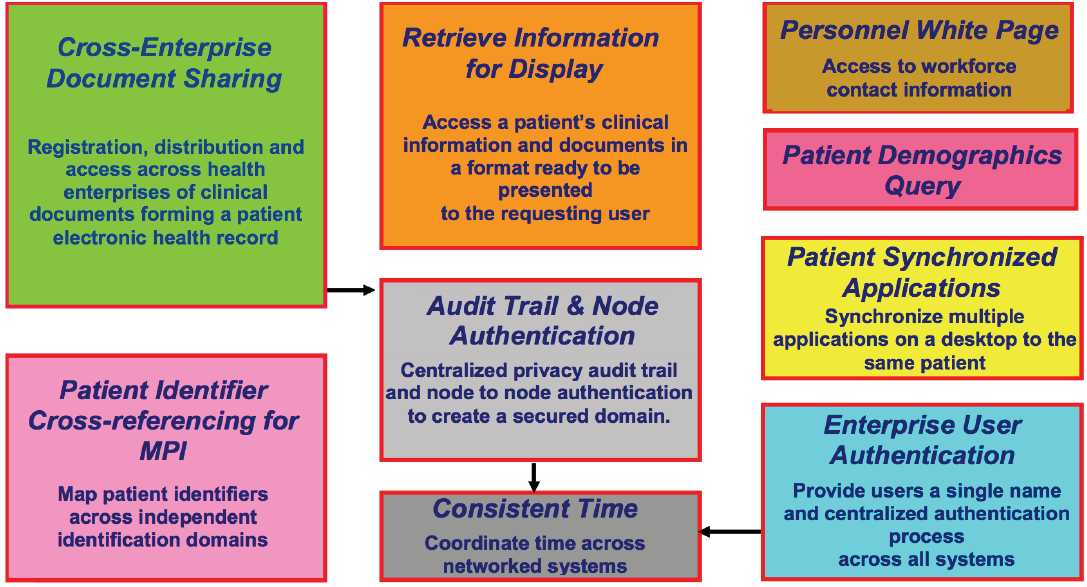
\includegraphics[width=150px]{img/ITI.png}
        \captionof{figure}{IHE IT Infrastructure Integration Profiles}
        \label{fig:IHE IT Infrastructure Integration Profiles}
\end{Figure}

\subsection{IHE Integrations Profiles (Extract)}
\begin{itemize}
   \item Audit Trail and Node Authentication (ATNA)
   \item Consistent Time (CT)
   \item Cross-Community Access (XCA)
   \item Cross-Community Patient Discovery (XCPD)
   \item Cross
\end{itemize}

\subsubsection{Consistent Time (CT)}
It is a timeserver, which provides a base-time. This is very important to make sure every transaction is based on the same time, especially to log all the different transaction (protocol) 
\begin{Figure}
   \centering
    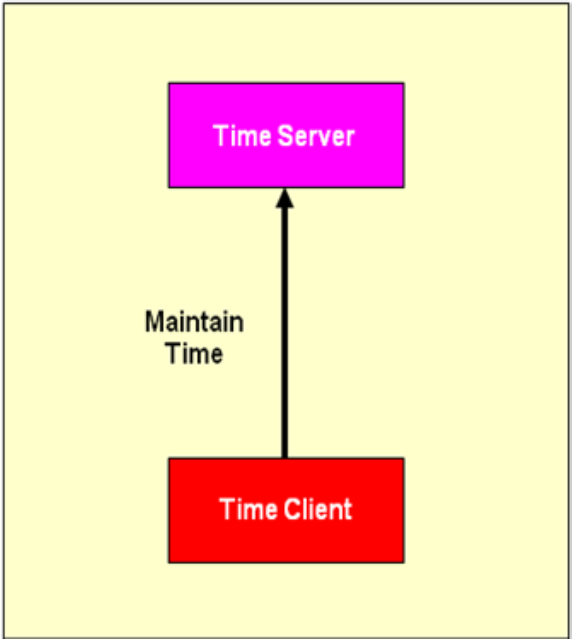
\includegraphics[width=150px]{img/CT.png}
        \captionof{figure}{Workflow from CT}
        \label{fig:Workflow from CT}
\end{Figure}

\subsubsection{Audit Trail and Node Authentication (ATNA)}
How interact every system with eachother and what have the different systems to provide
\begin{Figure}
   \centering
    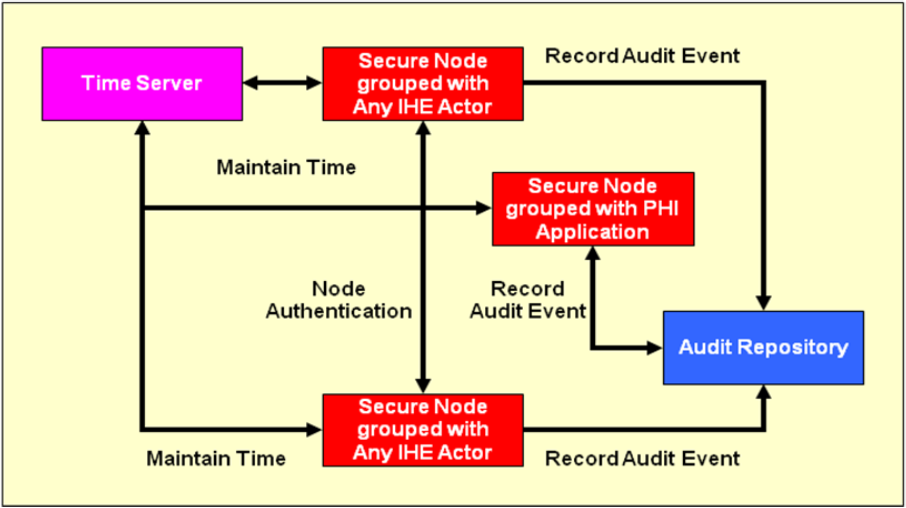
\includegraphics[width=150px]{img/ATNA.png}
        \captionof{figure}{Workflow from ATNA}
        \label{fig:Workflow from ATNA}
\end{Figure}

\subsubsection{Patient Identifier Cross-Referencing}
The PIXV3 Profile supports the cross-referencing of patient identifiers from multiple Patient Identifier Domains. These cross-referenced patient identifiers can then be used by 'identity consumer' systems to correlate information
about a single patient from sources that 'know' the patient by different identifiers. This allows a clinican to have more complete view of the patient information\\

\textbf{Important:} Within an EHR it is not allowed to use the 'social security number' (AHV-Nummer). Furthermore there is no national-identify-method for patient. Every hospital has its own ID-System for the patients

\begin{Figure}
   \centering
    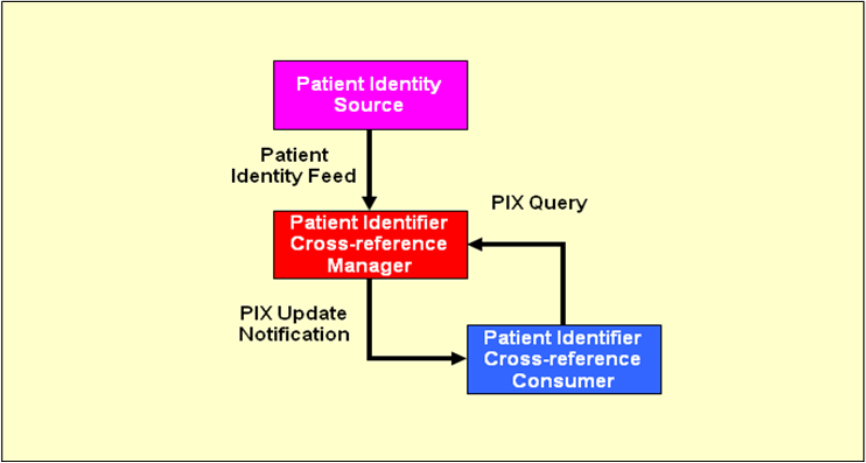
\includegraphics[width=150px]{img/PIX.png}
        \captionof{figure}{Workflow from PIX}
        \label{fig:Workflow from PIX}
\end{Figure}

A \textbf{Master Patient Index (MPI)} connects different ID's (e.g. from different hospital) to get one single ID
\begin{Figure}
   \centering
    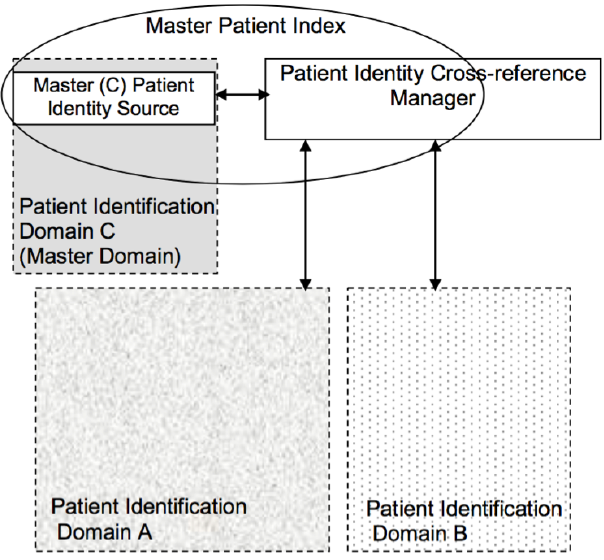
\includegraphics[width=150px]{img/MPI.png}
        \captionof{figure}{Workflow from MPI}
        \label{fig:Workflow from MPI}
\end{Figure}

\subsubsection{XDS Cross-Enterprise Document Sharing}
\begin{itemize}
   \item Cross-Enterprise Document Sharing enables a number of healthcare delivery organizations belonging to an XDS Affinity Domain (e.g. a community of care) to cooperate in the care of patient by sharing clinical records in the form of documents as they proceed
   \item ... tbd ... 
\end{itemize}

\begin{Figure}
   \centering
    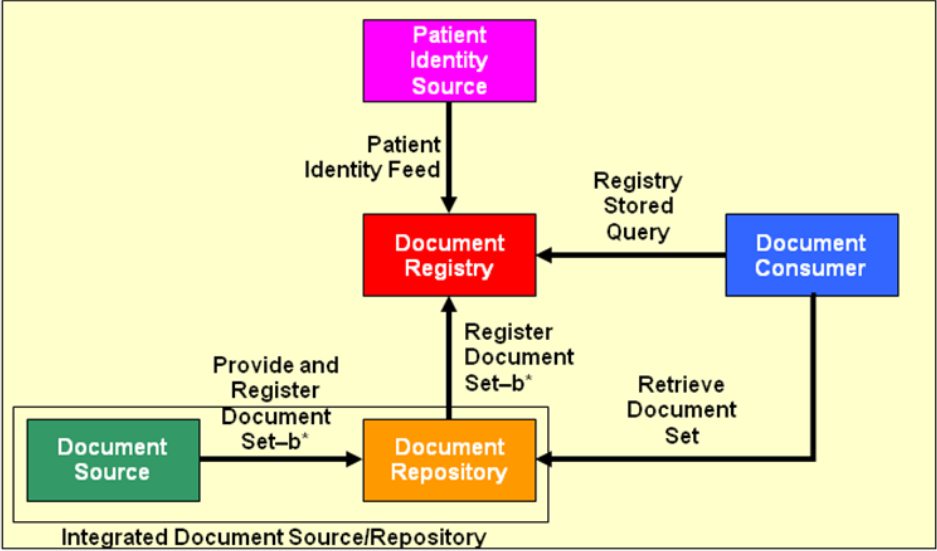
\includegraphics[width=150px]{img/XDSb.png}
        \captionof{figure}{Workflow from XDS.b}
        \label{fig:Workflow from XDS.b}
\end{Figure}

\textbf{XDS Affinity Domain}
An XDS Affinity Domain is a group of healthcare enterprises that have agreed to work together using a common set of policies and share a common Infrastructure

\begin{Figure}
   \centering
    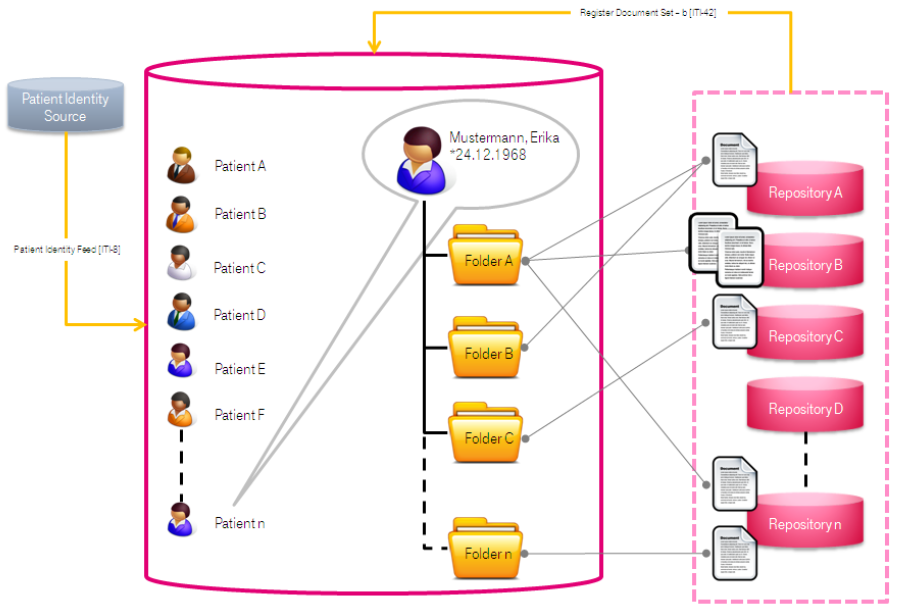
\includegraphics[width=150px]{img/DocumentRegistry.png}
        \captionof{figure}{Workflow to register a document}
        \label{fig:Workflow to register a document}
\end{Figure}

\begin{Figure}
   \centering
    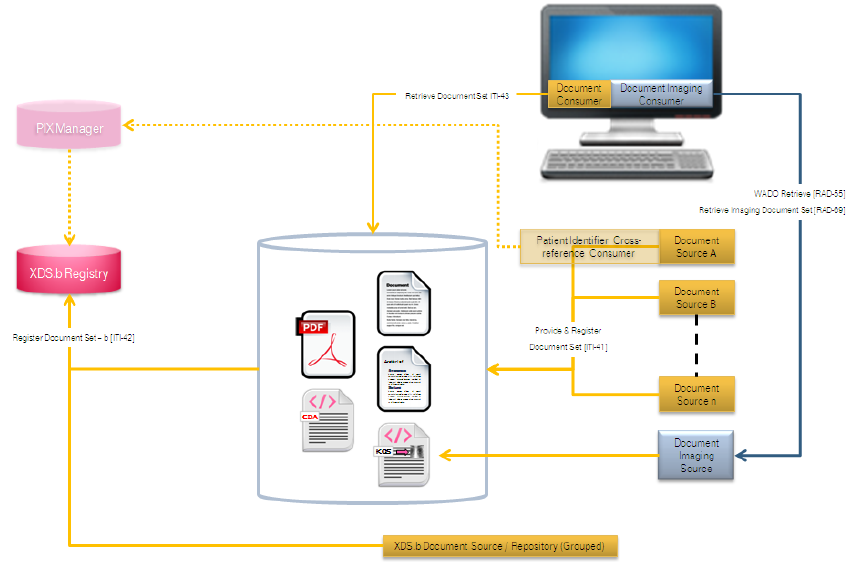
\includegraphics[width=150px]{img/DocumentRepo.png}
        \captionof{figure}{Workflow for a document-repository}
        \label{fig:Workflow for a document-repository}
\end{Figure}

\begin{Figure}
   \centering
    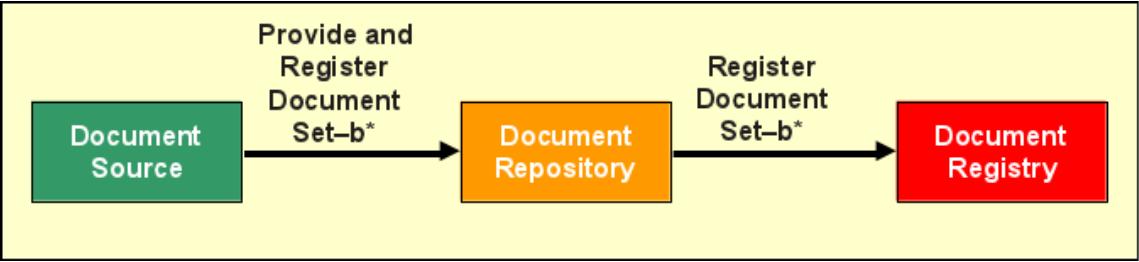
\includegraphics[width=150px]{img/ITI41.png}
        \captionof{figure}{Workflow from ITI-41}
        \label{fig:Workflow from ITI-41}
\end{Figure}

\textbf{XDS Concepts}
\begin{itemize}
   \item Submission Set
   \subitem is related to care event(s) of a single patient provided by the care delivery organization performing the submission request 
   \item Document
   \subitem will be stored in the repository 
   \item Metadata
   \subitem Data of the submission set and data of the document will be stored in the 
\end{itemize}

\begin{Figure}
   \centering
    
\includegraphics[width=150px]{img/ITI18.png}
        \captionof{figure}{Workflow from ITI-18}
        \label{fig:Workflow from ITI-18}
\end{Figure}

\begin{Figure}
   \centering
    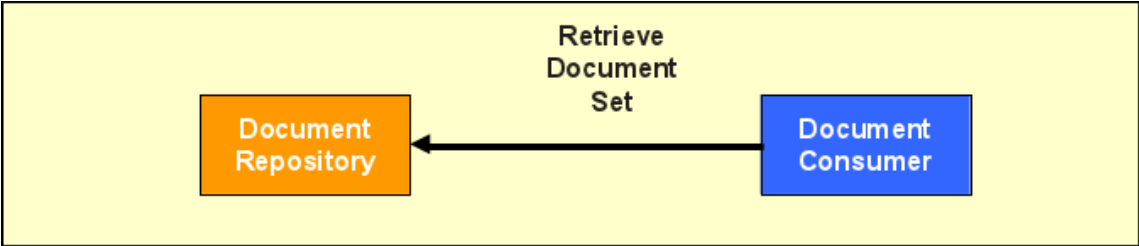
\includegraphics[width=150px]{img/ITI43.png}
        \captionof{figure}{Workflow from ITI-43}
        \label{fig:Workflow from ITI-43}
\end{Figure}

\chapter{EPR}
\begin{itemize}
   \item personal collection of documents relating to your health
   \item the healthcare professionals file these documets in your EPR
   \item you alone decied which healthcare professional may read which documents 
   \item you are not obliged to have an EPR. you can choose whether to have an EPR or not
   \item The Federal Act ont the Electronic Patient Record (EPRA) descripes how the EPR must be organised and technically secured
   \item 
\end{itemize}

\section{EPRA}
\begin{itemize}
   \item EPDG / EPRO
   \subitem Bundesgesetzt über das elektronische Patientendossier 
   \item EPDV
   \subitem Verordnung über das elektronische Patientendossier 
   \item EPDV-EDI (Stufe Department)
   \subitem Verordnung des EDI über das elektronische Patientendossier 
\end{itemize}

\begin{Figure}
   \centering
    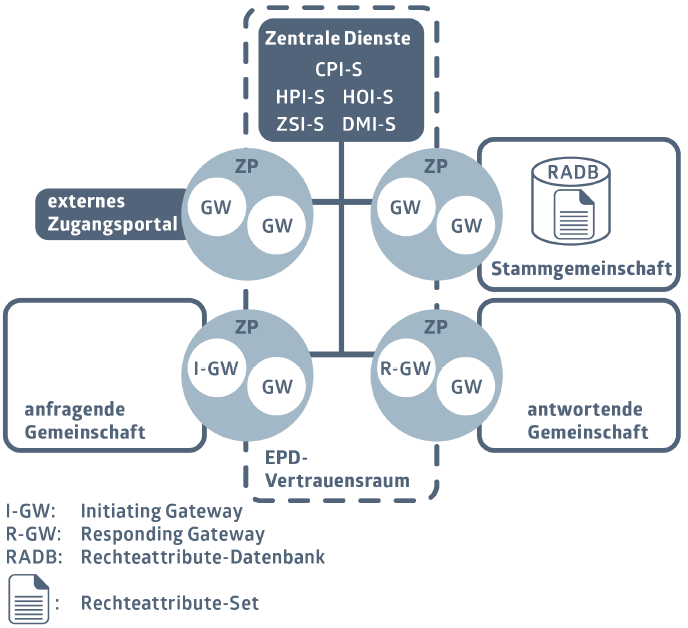
\includegraphics[width=150px]{img/EPRA.png}
        \captionof{figure}{Schema of EPR}
        \label{fig:Schema of EPR}
\end{Figure}


\chapter{Clinical Decision Support}

\section{Decision Support Systems - DSS}
\begin{itemize}
   \item computer-based information system that supports decision-making activities
   \item can be fully computerized or be part of the human computer interaction
   \item typically implemented as
   \subitem Decision trees
   \subitem Rule-based expert systems
   \subitem also: 'hard-coded' small, problem-speicific apps
   \subitem also: web apps, mobile apps, web-services $\rightarrow$ non-monolithic 
\end{itemize}

\subsection{Clincial Decision Making}
\begin{itemize}
   \item medical decision making required the clinician to apply accumulated knowledge to a specific amount of patient information to produce a result that may be a diagnosis, prognosis, cooruse of therapy or the selection of further tests
   \item $\Rightarrow$ Too often: the decisions are based on limited knowledge, the information is incomplete or imperfect and the decision must be made during a limited period of time
\end{itemize}

\subsection{Challenges of Medical Knowledge}
\begin{itemize}
   \item Knowledge multiplied faster and faster
   \item to err is human (Irren ist menschlich)
   \item Knowledge access and decision support at point of care
   \item Demand for change to increase quality and safety
\end{itemize}

\subsection{Decision Supportt today}
\begin{itemize}
   \item Many questions arise during patient care
   \item If they have questions they consider to
   \subitem to ask collegues
   \subitem do research in the internet
   \subitem use medical guidelines
   \subitem use medical handbooks
   \subitem search in bilbiographic retrieval systems (e.g. PubMed)
   \item $\Rightarrow$ These tools provde data needed, but they do not help to apply that information 
\end{itemize}

\section{Usage of CDSS}
\begin{itemize}
   \item passive Usage
   \subitem use when advice needed
   \subitem get recommendation by CDSS 
   \item active Usage
   \subitem gives advice automatically under certain conditions
   \subitem user evalute the advice and accept/reject it
   \subitem $\Rightarrow$ alert fatique 
\end{itemize}

\subsection{Further challanges}
\textbf{Transformation}
\begin{itemize}
   \item from reactive to proactive and preventive care
   \item from clinical-centric to patient-centered practice
   \item from training-based interventions to aggregated evidence
   \item from episodic response to continuous health monitoring
\end{itemize}
\textbf{eHealth Opportunities}
\begin{itemize}
   \item Data-driven evidence
   \item Big Data
   \item information and knowledge management
   \item hybrid intelligence $\rightarrow$ machine and human intelligence
\end{itemize}

\section{Clinical Decision Support - CDS}
\textbf{Definition:} \textit{A clinical decision support system is any computer program designed to help health professionals make clinical decisions, deal with medical data about patients or with the knowledge of medicine necessary to inerpret such data}\\
This can be classify into
\begin{itemize}
   \item tools for knowledge management
   \item tools for focusing attention
   \item tools for patient-specific consultation
\end{itemize}
$\Rightarrow$ CDS systems should identify and reduce the rate of errors, inappropriate actions and adverse events
\begin{itemize}
   \item reduced medication errors
   \item decreased costs
   \item alert and reminders e.g. drug-drug interaction
\end{itemize}

\section{Decision Support Systems in Hospitals}
\textbf{Clinical}
\begin{itemize}
   \item Medical Knowledge Management
   \item Vital Sign Alerts
   \item Recommendations
   \item Lab and Medication Checks
\end{itemize}
\textbf{Administrative}
\begin{itemize}
   \item Management Cockpits
   \item Data Mining (BI in Health Care)
   \item Quality Assurance
\end{itemize}

\begin{Figure}
   \centering
    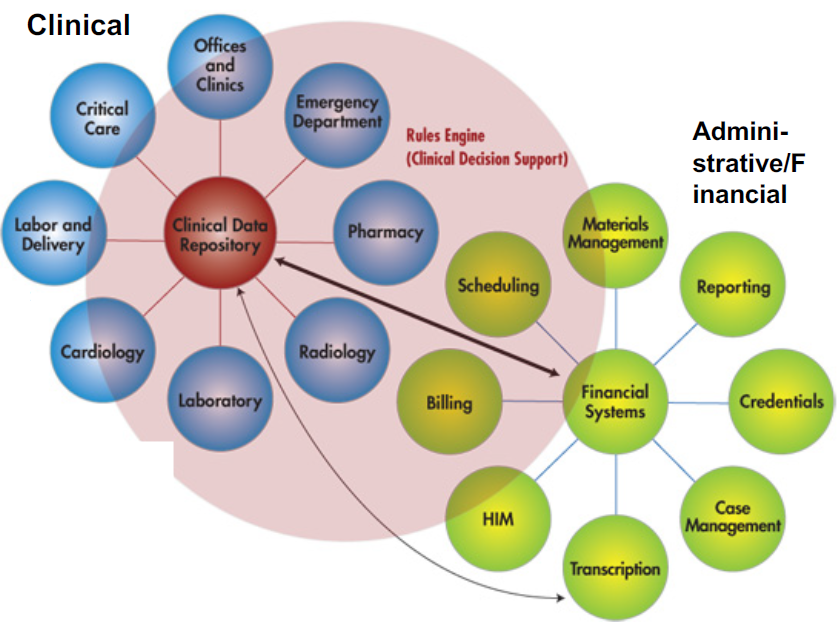
\includegraphics[width=150px]{img/DCSS.png}
        \captionof{figure}{Decision Support Systems in Hospitals}
        \label{fig:Decision Support Systems in Hospitals}
\end{Figure}

\subsection{Basic components}
\begin{itemize}
   \item Medical ontology $\rightarrow$ standardized vocabulary
   \item Knowledge Base (KB) $\rightarrow$ set of rules, condition actions, IF-Then Rules, constraints
   \item Fact base $\rightarrow$ working memory, prefilled with data from patient's EHR
   \item Inference engine $\rightarrow$ constantly apply rules of KB on working memory, does react on recognized conditions by an action
\end{itemize}

\subsection{CDS applications}
\begin{itemize}
   \item alerts and reminders $\rightarrow$ lab results, medication etc.
   \item Image recognition and interpretation
   \item Diagnostic assistance
   \item therapy critiquing and planning
   \item clinical guidelines
   \item condiiton-specfific order sets
   \item generation of patient data reports
\end{itemize}

\subsubsection{Decision Trees}
\begin{itemize}
   \item basic knowledge representation for logical decisions
   \item natural order of micro decisions to reach a conclusion
\end{itemize}

\begin{Figure}
   \centering
    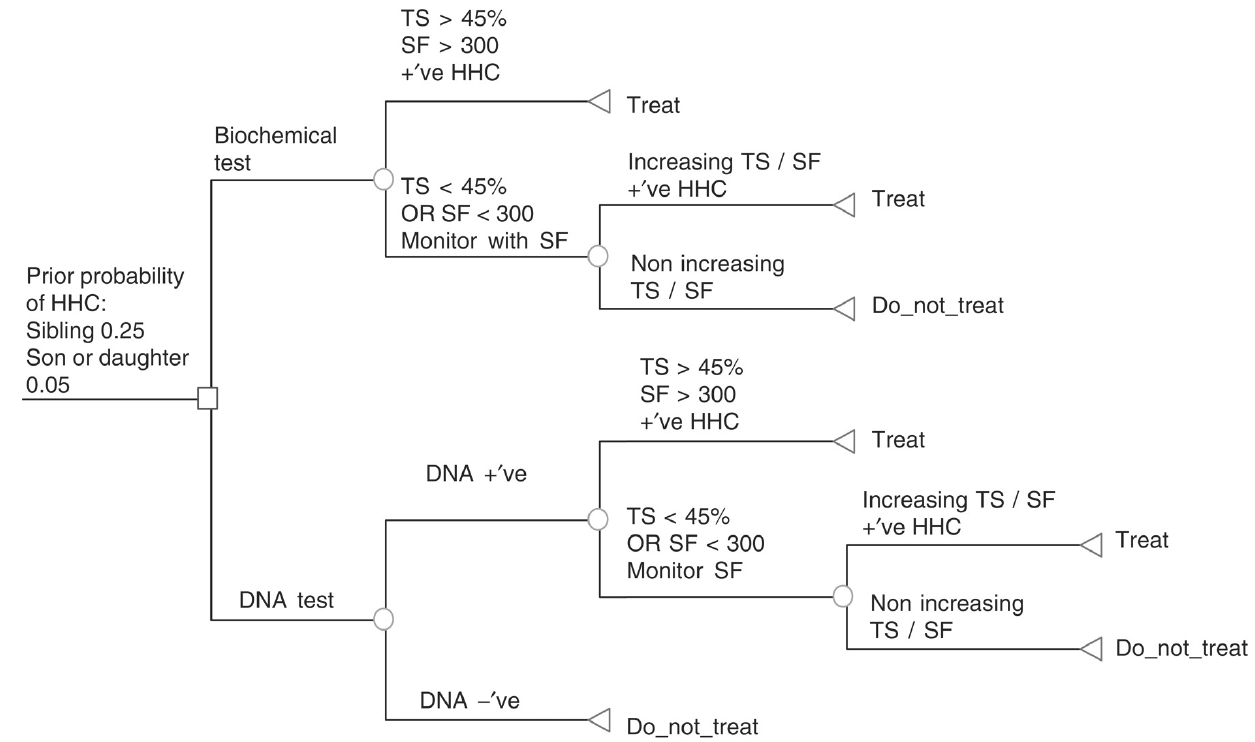
\includegraphics[width=150px]{img/DecisionTree.png}
        \captionof{figure}{example decision tree}
        \label{fig:example decision tree}
\end{Figure}

\subsection{CDSS for real-time intervention}
CDSS as \textit{active knowledge systems} using case-specific patient data are designed to remind the physician
\begin{itemize}
   \item flag abnormal values
   \item provide explanation for these abnormals
   \item alert possible drug interactions or incorrect drug dosages
   \item recommendation about additional tests and examinations
   \item advices on treatment
\end{itemize}

is triggered By
\begin{itemize}
   \item Task (data entry, data review, workflow) $\rightarrow$ dose range checks, drug-drug interaction \dots
   \item Event (data-driven) $\rightarrow$ Monitoring Alerts, Pager alerts on abnormal lab results
   \item Time (reminders)
\end{itemize}

\subsection{The five rights of CDS}
CDS intervention should provide
\begin{enumerate}
   \item the \textbf{right information} $\rightarrow$ evidence based guidance, response to clinical need
   \item to the \textbf{right person} $\rightarrow$ entire care team - including the patient
   \item through the \textbf{right channels} $\rightarrow$ e.g. EHR, mobile device \dots
   \item in the \textbf{right formats} $\rightarrow$ e.g. order sets, dashboards \dots
   \item at \textbf{right time} $\rightarrow$ for key decision or action
\end{enumerate}

\subsection{Challenge in building a CDSS}
\textbf{Technical}
\begin{itemize}
   \item Complexity of CDSS: Editor, Knowledge Base, Engine
   \item Knowledge acquisition: espensive to develop and maintain KB
   \item System integration: workflow, UI
\end{itemize}

\textbf{non-technical}
\begin{itemize}
   \item cultural issues and user resistance
   \item incompatibility among approaches
   \item Human factors $\rightarrow$ not matching the five right and alert fatique
\end{itemize}

\subsection{CDS Standards}
$\rightarrow$ HL7 Standards from Health eDecisions (HeD)
\begin{itemize}
   \item Virtual Medical Record (vMR) data model
   \item CDS Knowledge Artifact Specification (KAS)
   \item Decision Support Service (DSS) Spec and IG
\end{itemize}

aligned with other relevant standards
\begin{itemize}
   \item vMR: CCD, CCDA, QRDA, Infobutton
   \item KAS: Order Set DSTU, GELLO, Arden, CDS, Consortium
   \item DSS: Infobutton, IHE Request for Clincal Guidance
\end{itemize}

\subsubsection{Arden}
\textbf{Syntax}
\begin{itemize}
   \item first approachto knowledge standardization
   \item Medical Logic Modules (MLMs)
   \subitem Each MLM contains maintenance information, links to other sources of knowledge and enough logic to make a signle health decision
   \subitem is a stram of text stored in an ASCII file
   \item MLM are working within host systems
   \subitem Input: an input parameter can be committed
   \subitem curly brace expressions: dynamic interaction between MLMs and host systems (map values to host system)
   \subitem Write Statements: texts can be written to host system
   \subitem Output: Commit from MLM after execution of MLM 
\end{itemize}

\textbf{MLM - Medical Logic Module}
Composed of slots, grouped into four categories
\begin{itemize}
   \item Maintenance
   \item Library
   \item Knowledge
   \item Resources
\end{itemize}

\begin{Figure}
   \centering
    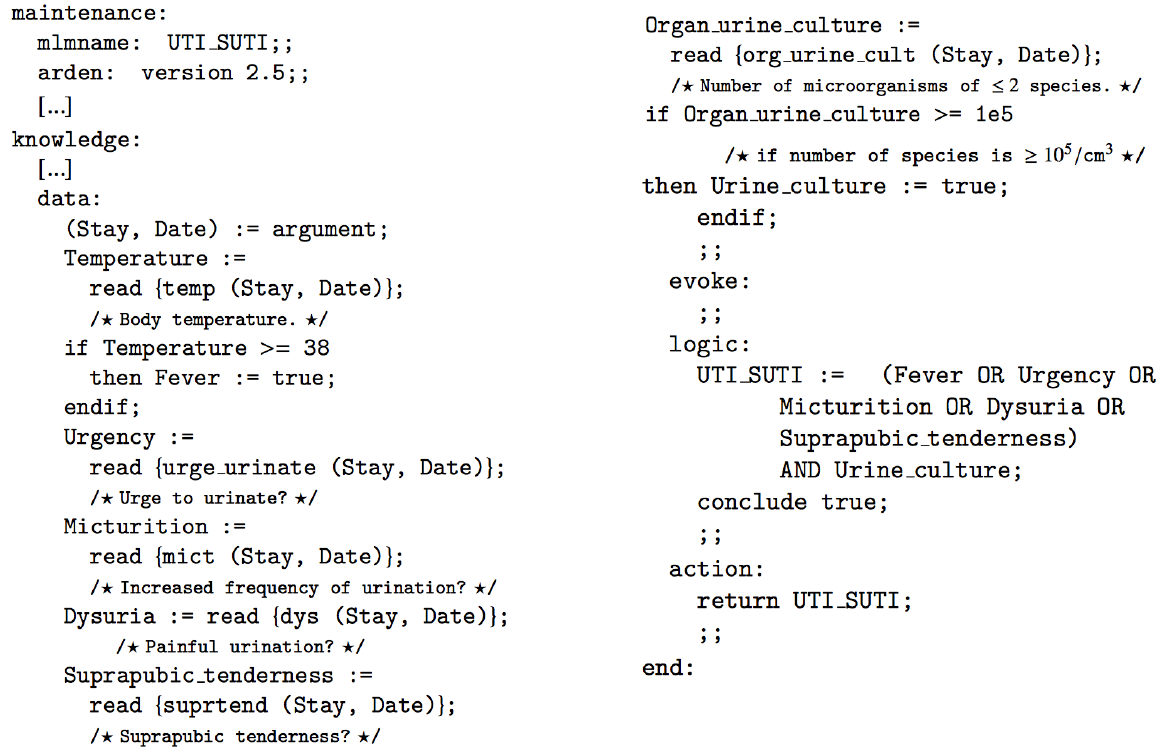
\includegraphics[width=150px]{img/MLMExample.png}
        \captionof{figure}{example MLM}
        \label{fig:example MLM}
\end{Figure}

\textbf{Fuzzy Arden Syntax}
\begin{Figure}
   \centering
    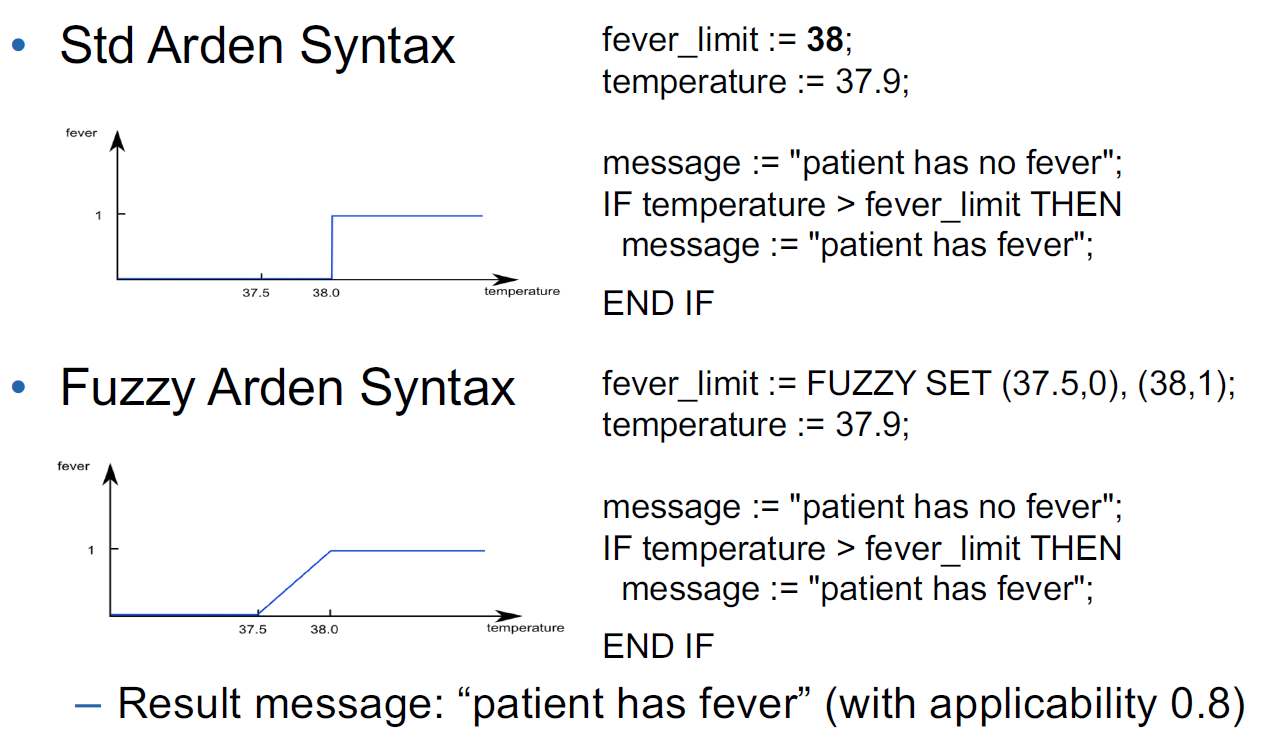
\includegraphics[width=150px]{img/FuzzyArdenSyntax.png}
        \captionof{figure}{The Fuzzy Arden Syntax}
        \label{fig:The Fuzzy Arden Syntax}
\end{Figure}

\textbf{Guidelines}
\begin{itemize}
   \item Much Development of guidelines since 70s
   \item Recent efforts aimed at computer-based interpretation
   \subitem Goal of delivering patient-specific recommendations at point of care
   \subitem Guidelines as core technology for many decision support applications
\end{itemize}

\textbf{Guideliens as a core technology}
\begin{itemize}
   \item protocol-based care
   \item chronic disease management
   \item consultations
   \item critical pathways, utilization review (UR) monitoring
   \item Referral management
   \item workflow / process optimization
   \item Infobuttons
   \item education and training
\end{itemize}

\subsubsection{HL7 CDS Standardization Work}
focusing on common Infrastructure
\begin{itemize}
   \item vMR: an object-oriented virtual medical record subset for decision support
   \item GALLO: object-oriented query and expression language
   \item Vocabulary management tools
   \item Taxonomy of services invoked by rules
\end{itemize}

\chapter{Medical Imaging Modalities}

\section{Imaging in Clinics}
\textbf{Clinical questions}
\begin{itemize}
   \item Anatomy: 
   \subitem Presence and localisation of lesions
   \subitem malformations
   \subitem internal bleedings
   \subitem fluid accumulation
   \item Physiology / Pathophysiology
   \subitem Energy consumption
   \subitem metabolism
   \subitem drug distribution
   \subitem blood flow 
\end{itemize}

\textbf{Medical context}
\begin{itemize}
   \item Localisation during surgery
   \item treatment planning
   \item screening
\end{itemize}

\textbf{Techniques and needed image information}
\begin{itemize}
   \item native tissue contrast (2D grey values)
   \subitem bone fractures (X-ray)
   \subitem soft tissue (CT, MRI, US) 
   \item static images with contrast media , e.g. x-ray (2D) CT angioraphy (2D or 3D), contrast MRI or US
   \subitem enhanced visibility of structures such as vessels
   \item time-resolved images (4D)
   \subitem cardio-CT
   \subitem organ motions (radiation treatment planning)
   \item Physiology / Pathophysiology
   \subitem time resolved image seriess with contrast media for blood Flow
   \subitem visualisation of metabolosim by uptake of radioactive tracers
   \item treatment planning for radiation therapy
   \subitem X-ray absorbtion measurements by CT allows electron density calculation
\end{itemize}

\subsection{Radioactive Decay}

\begin{equation}
   \frac{dN}{dt} = - \lambda N
\end{equation}


\chapter{3D Human Body Visualization}

\section{Application of Medical Visualization}
\begin{itemize}
   \item visual data exploration
   \item virtual autopsy $\rightarrow$ patient (in original size) lying on the table to be analyzed
   \item Multimodel visualization $\rightarrow$ Overlay of PECT/CT data
   \item Surgical planning with virtual models
   \item Using for printing 3D models
   \item Computer assisted surgery $\rightarrow$ da-vinci robot
   \item radiation therapy planning
   \item medical illustration
   \item anatomy training
   \item surgical training
\end{itemize}

\section{DICOM Standards}
\begin{itemize}
   \item \textbf{D}igital \textbf{I}maging \textbf{Co}mmunications in \textbf{M}edicine
   \item Covers most image formats for medical application
   \item specification for messaging and communication between imaging machines 
\end{itemize}

\begin{Figure}
   \centering
    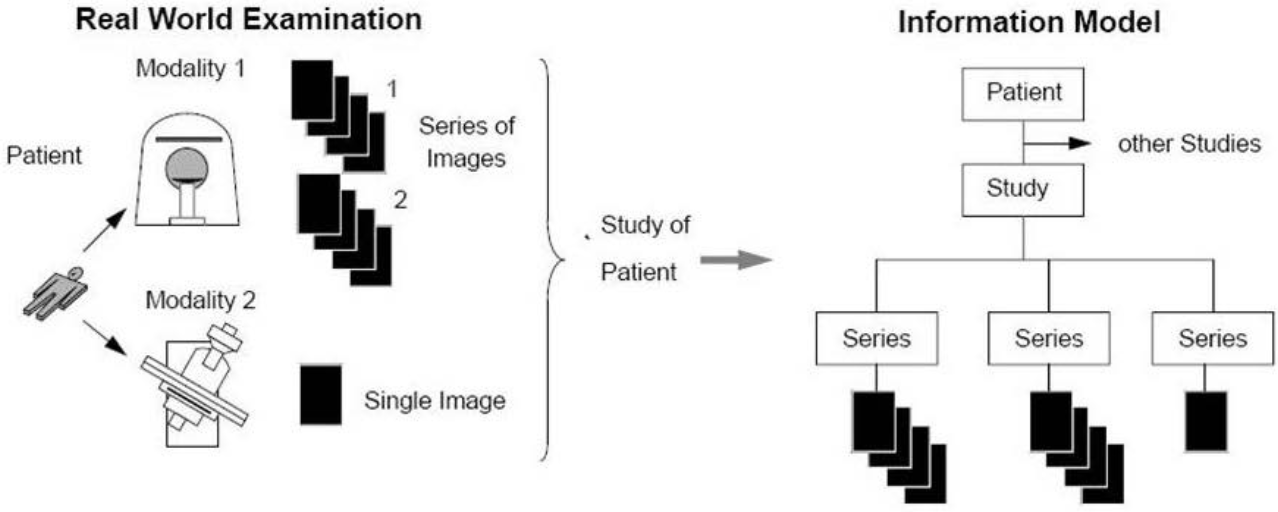
\includegraphics[width=150px]{img/DICOM.png}
        \captionof{figure}{DICOM Information Model}
        \label{fig:DICOM Information Model}
\end{Figure}

\subsection{Modalities}
\begin{itemize}
   \item Radiation (x-rays)
   \item Computer Tomography (CT)
   \item Magentic Resonance Imaging (MRI)
   \item Ultrasound (US)
   \item Positron Emission Tomography (PET)
   \item Single Photon Emission Computed Tomography
   \item Optical
\end{itemize}

\subsection{Coordinate Systems}
\begin{Figure}
   \centering
    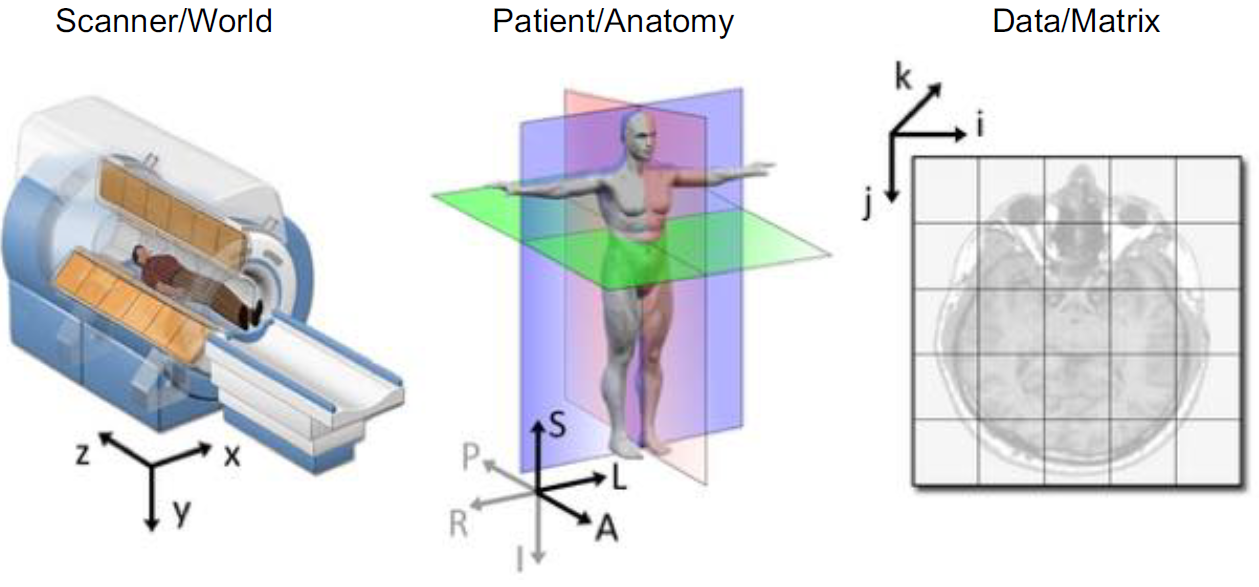
\includegraphics[width=150px]{img/CoordinateSystems.png}
        \captionof{figure}{Coordinate Systems}
        \label{fig:Coordinate Systems}
\end{Figure}

\subsection{Orientation}
\begin{Figure}
   \centering
    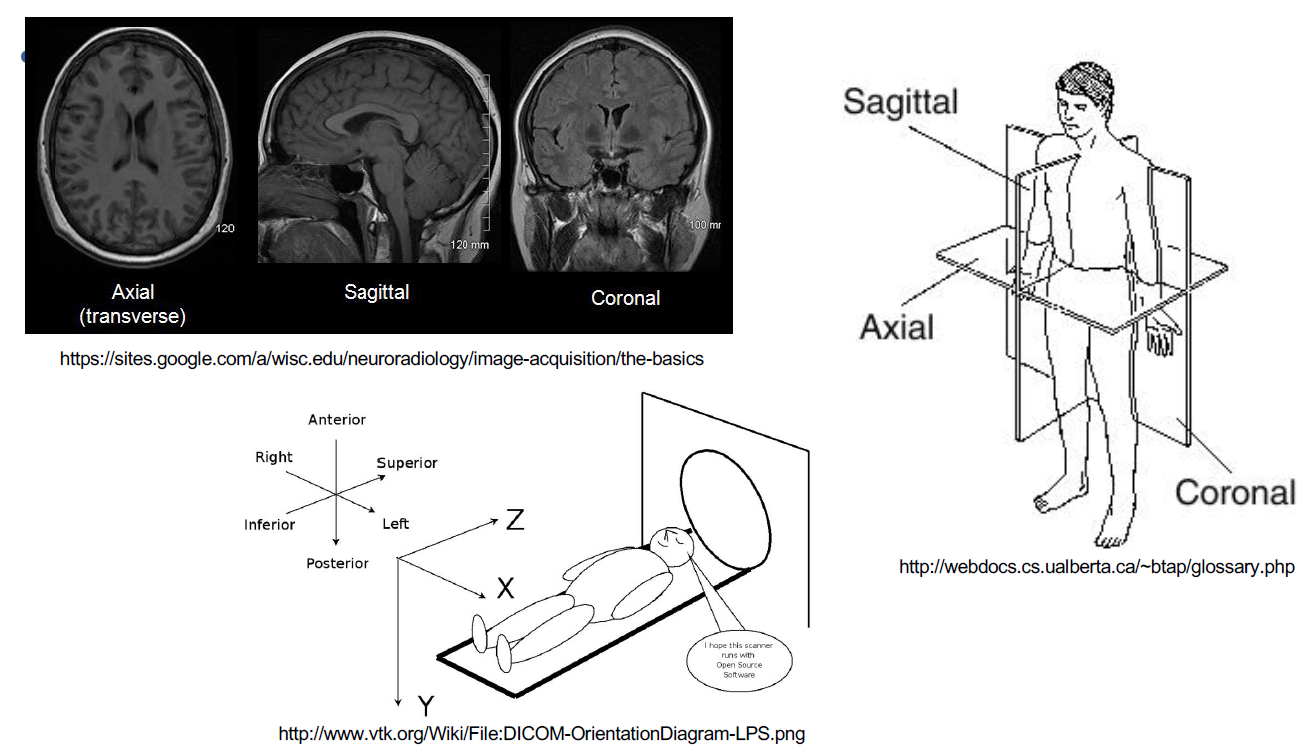
\includegraphics[width=150px]{img/Orientation.png}
        \captionof{figure}{Orientation}
        \label{fig:Orientation}
\end{Figure}

\subsection{Visualization Modes of Medical Images}
\begin{enumerate}
   \item Extract slices to display 2D image
   \item Use transfer function and perform direct volume rendering
   \item generate a polygonal model to render surface
\end{enumerate}


\chapter{Introduction to Semantic Web Technologies}

To query the data we can use SPARQL - it is really similar to SQL but there is e.g. no join-function. \\
Baseline for the queries are the graph database model
\begin{itemize}
   \item easy to interlink and extend
   \item Data usuallry stored as triples in RDF (Resource Descirption Framework)
   \item Triple = <subject, predicate, object>
   \subitem e.g. "<gene X>isExpressedIn<anatomic enitity Y>"
   \subitem in SPARQL $\rightarrow$ Select * where \{?gene isExpressedIn ?anatEntity\}
   \item tto: tutorial object
   \item ttr: tutorial resource
\end{itemize}

\section{Semantic Web Technology Stack}

\begin{Figure}
   \centering
    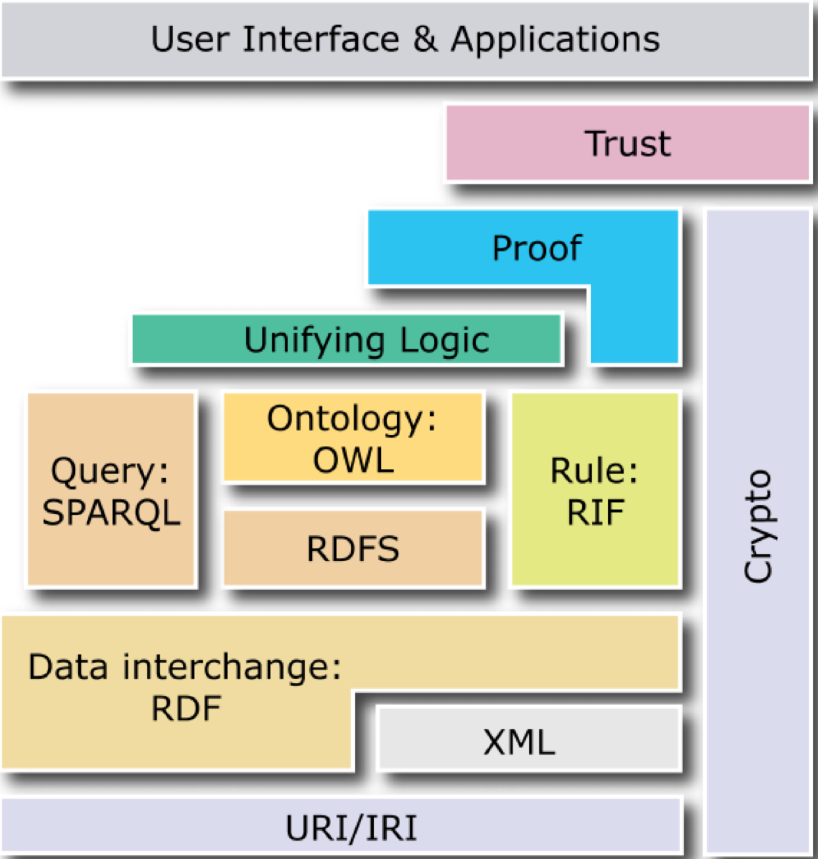
\includegraphics[width=150px]{img/SemanticWebTechStack.png}
        \captionof{figure}{Semantic Web Technology Stack}
        \label{fig:Semantic Web Technology Stack}
\end{Figure}

\subsection{Ontology}
\textit{What is an ontology?}
\begin{itemize}
   \item a model of a domain
   \item A vocabulary consisting of classes and properties
   \item Machine-readable knowledge representation
\end{itemize}

\textit{How do we build one?}
\begin{itemize}
   \item Descripe new classes and properties
   \item Extend existing ontologies (RDF schemas, dbpedia, ...)
\end{itemize}

\begin{Figure}
   \centering
    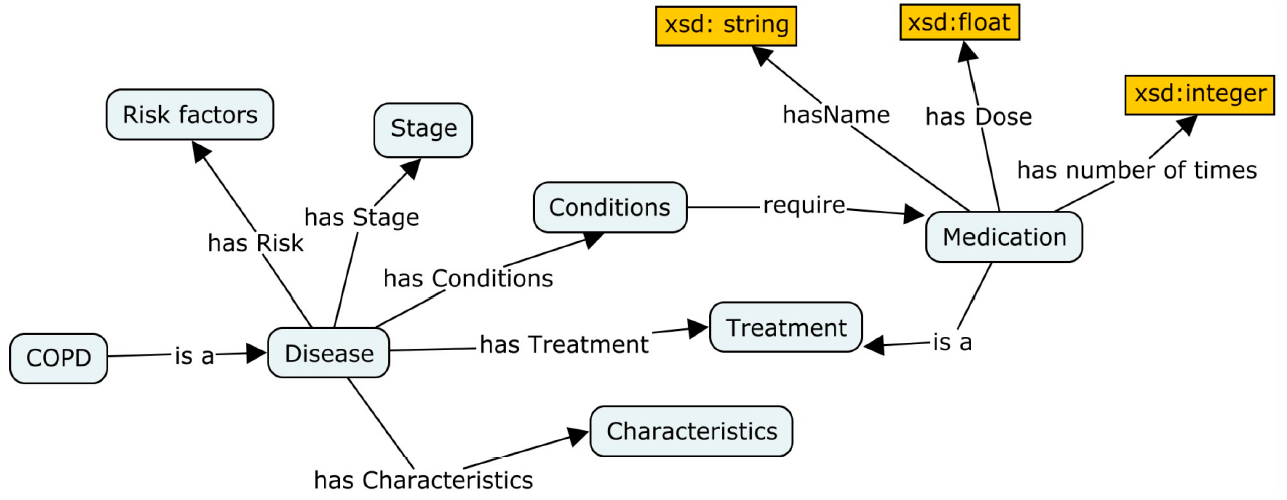
\includegraphics[width=150px]{img/simpleOntology.png}
        \captionof{figure}{Simple Ontology}
        \label{fig:Simple Ontology}
\end{Figure}

\subsubsection{Why data integration?}
\begin{itemize}
   \item Study diseases across species
   \subitem e.g. using model organisms (mice) to understand / predict evolution of disease in humans 
   \item Repurpose drugs
   \subitem Prioritise existing drugs for new diseases $\leftrightarrow$ reducing time and cost for devel 
   \item Understand gene function 
   \subitem E.G. what genes have a role in respiration?
   \subitem What genes are associated with possible cancer types? 
\end{itemize}

It is very important to build precise queries. For example the term 'rich' can be interpreted differently. e.g. Bill Gates has another understanding in rich, so it won't be a good idea to set the question 'which employees are rich?'


\chapter{mobile Health}
eHealth + mobile = mobile health = mHealth

\section{Telemedicine}
Telemedice provides clinical health care from a distance using ICT, this includes:
\begin{itemize}
   \item Telehealth / Teleconsultation (via teleconferencing)
   \subitem Phone and Video Conferencing 
   \item mobile health
   \subitem Smartphones, smartwachtes, wearables 
   \item Remote monitoring
   \item Outsourced speciality care as digital services
   \subitem Tele-cardiology, -psychiatry, -dentristry, \dots
   \subitem Integrated via digital networks 
\end{itemize}

\subsection{in Practice: Medgate AG}
\begin{itemize}
   \item leading provider of integrated healthcare services in Switzerland
   \item Up to 6000 teleconsultations a day
   \item Up to 2.5 million patient records
   \item Teleconsultation
   \subitem Communication channels: telephone, internet, video, App 
   \item Telediagnostics
   \subitem diagnosis of images
   \subitem telemonitoring 
   \item Teletherapy
   \subitem prescirption of drugs
   \subitem sick leave certificates 
   \item Medgate App
\end{itemize}

\section{mHealth Expactations}
$\rightarrow$ Healthcare is everywhere

\begin{itemize}
   \item smartphone is part of our life
   \subitem Smartphones are always on, computers are not 
   \item eHealth at any point of care
   \subitem at home / work / bedside etc. 
   \item telemedicine services
   \subitem Remote health serices in rural regions
   \subitem health services for developing countries 
   \item Patient engagement
   \subitem increased self-management of well-being and illness
   \subitem reduced number of hospital stays 
\end{itemize}

\begin{Figure}
   \centering
    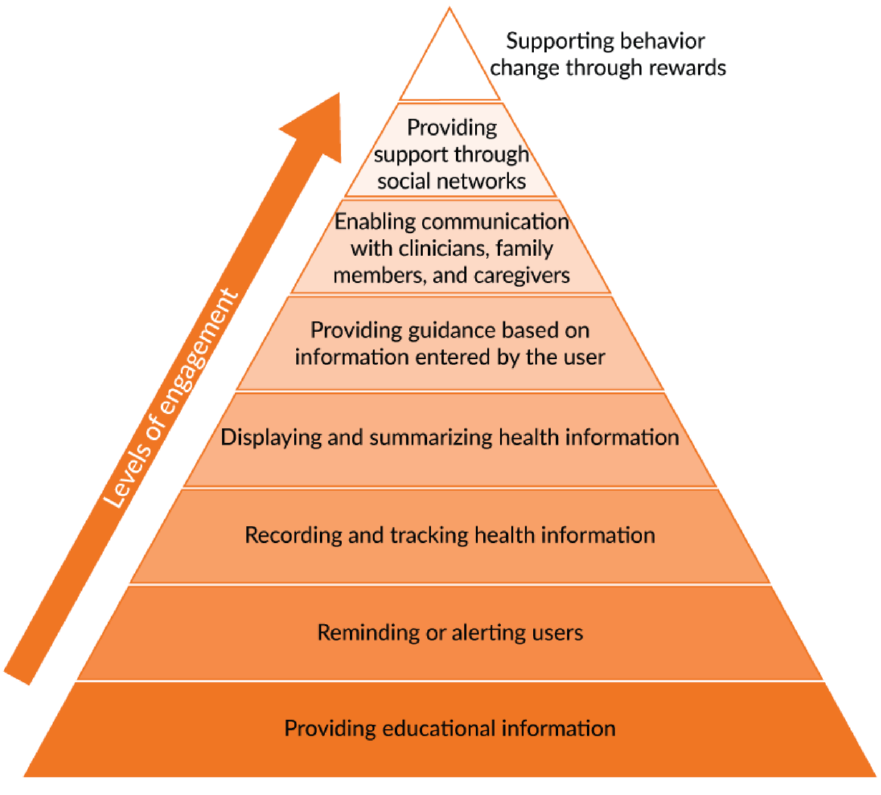
\includegraphics[width=150px]{img/EngagementApps.png}
        \captionof{figure}{Patient Engangement using Apps}
        \label{fig:Patient Engangement using Apps}
\end{Figure}

\subsection{Types of mHealth Apps}
\begin{itemize}
   \item Clinical assistance apps
   \item Reference / database apps (eg.UpToDate)
   \item General facility information / communication apps
   \item Monitoring apps (telemedicine)
   \item Reminder apps (e.g., medication)
   \item healthy life apps (fitness, nutrition, diets, mood)
   \item patient portal / EHR apps
   \item speciality / disease-specific apps (pregnancy, kids, diabetes)
\end{itemize}

$\Rightarrow$ most apps re for patients / consumers, not for healthcare professionals

\section{mHealth today}
\begin{itemize}
   \item Large number of lifestyle, fitness and well-being apps
   \subitem no clear evidence on their quality and reliability 
   \item Role of mHealth in healthcare systems unclear
   \subitem Personal vs. clinical mHealth apps, business models 
   \item Issues on privacy and security
   \subitem a lot of free Apps
   \subitem Regulations and laws are not (yet) established 
   \item Standards, protocols and guidelines are evolving
   \subitem importance of sharing and transfering best practices 
   \subitem need for certification schemes / quality labelling 
\end{itemize}

\subsection{mHealth Challenges}
\begin{Figure}
   \centering
    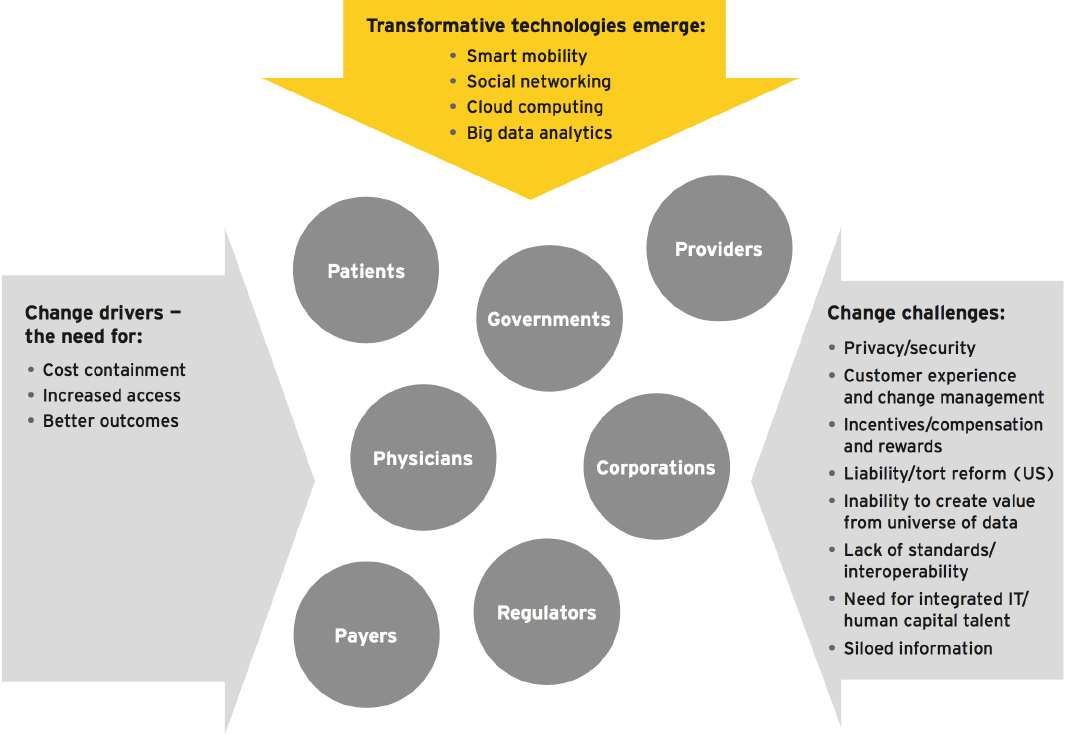
\includegraphics[width=150px]{img/mHealthChallenges.png}
        \captionof{figure}{eHealth and mHealth Challenges today}
        \label{fig:eHealth and mHealth Challenges today}
\end{Figure}

\subsection{eHealth App Regulation}
\begin{itemize}
   \item International regulations
   \subitem US: FDA, Health Insurance Portability and ACcountability Act (HIPAA) Security Rule
   \subitem EU: Medical Device Regulation (MDR)
   \item National regulations in CH
   \subitem Datenschutzgesetz (DSG), Datenschutzverordnung
   \subitem Heilmittelgesetzt (HMG), Medizinprodukteverordnung (MepV) $\rightarrow$ Anlehnung an EU-Richtlinien
   \item Guidelines
   \subitem App Store Review Guidelines
   \item Recommendations  
\end{itemize}

$\Rightarrow$ \textit{Is an eHealth App a Medical Device?}\\
\textbf{EU MEDDEV regulations}
\begin{itemize}
   \item Hospital Information Systems are not qualified as medical devices. However they may be used with additional modules which might be qualified in their own right as medical devices
   \item EHR systems that simply replaces a patient's paper file does not meet the definition of a medical device. But certain modules can be a medical device
   \item Modules that contribute to diagnosis, therapy and follow-up (e.g. generate alarms) are qualified as medical devices
   \item Decision Support Software are qualified as medical devices
\end{itemize}

\subsubsection{Apple App Store Guidelines}
$\Rightarrow$ Strict rules for health and wellness apps
\begin{itemize}
   \item privacy protection
   \item avoid physical harm
   \subitem Inaccurate data that could potentially cause physical harm
   \subitem Apps related to forbidden drugs
   \subitem Apps with harmful recommendations
   \item Drug dosage calculators must come from the drug manufacturer, a hospital, university, health insurance company, or other approved entity, or receive approval by the FDA or one of its international counterparts
\end{itemize}

\textit{What does this mean?}
\begin{itemize}
   \item Laws and reulgations are currently work in progress
   \item If a software is a medical product / medical device
   \subitem I) A CE certification is need
   \subitem II) The software company has to run a documented software quality management process (eg. ISO 13485)
   \item App store might reject your app 
\end{itemize}


\section{Sustainable eHealth Apps}

\begin{itemize}
   \item Legal and ethical
   \item Financial
   \item Clinical
   \item Technological
   \item Integrated
   \item Personalized
\end{itemize}

\section{mHealth App Functionalities}
\begin{itemize}
   \item Data capture
   \item Data Analysis
   \item Sense making
   \item Data sharing
\end{itemize}

\section{Patient Generated Data}

\begin{itemize}
   \item Behavioral characteristic
   \subitem Self-monitored vital data
   \subitem physical activity
   \subitem eating patterns / risky drinking
   \subitem medication taking
   \subitem sleep quality
   \item Psycho-social characteristic
   \subitem Mood and stress
   \subitem anxiety and depression
   \subitem quality of life symptoms (Pain free, headaches, migraine etc.)
\end{itemize}


\chapter{mHealth Wearables}

\section{Health Devices at Home}
There are two main topics
\begin{itemize}
   \item Smart Homes
   \subitem Digital weighing Scale
   \subitem Air quality sensors 
   \item Ambient-Assisted Living (AAL)
   \subitem automated wireless and fixed monitoring and assistance to help people cope with age-related limitations
   \subitem speech-recognition devices
   \subitem cameras
   \subitem floor sensors
   \subitem smart furnitures
   \subitem urine monitors
\end{itemize}

\subsection{AAL}
Assisted Living + Ambient Intelligence $\rightarrow$ Assisted living technologies for older adults. This is possible through different field in Technologies:
\begin{itemize}
   \item Smart homes
   \item mobile devices
   \item wearable sensors
   \item smart fabrics
   \item assistive robotics
\end{itemize}
$\rightarrow$ Sensors and actuators integrated into everyday objects

\subsubsection{Health Monitoring and Smart Homes}
\begin{itemize}
   \item Ambient
   \subitem Room temperature
   \subitem air quality
   \subitem weather condition
   \subitem air pollution
   \subitem pollen concentration in the air
   \item Surveillance
   \subitem movement
   \subitem behaviour
\end{itemize}

\chapter{Glossary}
has to be done
Fachbegriffe 
PIS
CIS
HIS
EHR
etc...

\begin{itemize}
   \item CDS - Clincial Decision Support
   \item DSS - Decision Support Systems
   \item CDSS - Clinical Decision Support Systems
   \item Computerized Clinical Decision Support
   \item Medical Decision Support
   \item MDSS - Medical Decision Support Systems
   \item CPOE - Computerized Provider Order Entry
   \item DRC - Dose range checks
   \item DDI - Drug-drug interaction
   \item HeD - Health eDecisions
   \item vMR - virtual medical Record
   \item KAS - Knowledge Artifact Specification
   \item MLM - Medical Logic Modules
   \item AAL - Ambient Assisted Living
\end{itemize}


\end{document}